\documentclass[UTF8,a4paper,12pt,fontset=none]{ctexart}

\usepackage[a4paper,margin=2.2cm]{geometry}
\usepackage{array}
\usepackage{booktabs}
\usepackage{caption}
\usepackage{enumitem}
\usepackage{float}
\usepackage{fontspec}
\usepackage{graphicx}
\usepackage{hyperref}
\usepackage{listings}
\usepackage{siunitx}
\usepackage{subcaption}
\usepackage{tabularx}
\usepackage{tikz}
\usepackage{xcolor}

\hypersetup{colorlinks=true,linkcolor=blue!60!black,urlcolor=blue!60!black}
\defaultCJKfontfeatures{AutoFakeSlant=.2}
\setCJKmainfont{Songti SC}
\setCJKsansfont{Heiti SC}
\setCJKmonofont{Heiti SC}
\setmonofont{Menlo}
\setlength{\parindent}{2em}
\setlength{\parskip}{0.35em}
\graphicspath{{../results/figures/}}
\captionsetup{font=small}
\sisetup{round-mode=places,round-precision=3}
\renewcommand{\figurename}{图}
\renewcommand{\tablename}{表}

\definecolor{AccentA}{HTML}{0B6E4F}
\definecolor{AccentB}{HTML}{1D4E89}
\definecolor{AccentC}{HTML}{F4A259}
\definecolor{AccentD}{HTML}{C73E1D}
\definecolor{CodeBg}{HTML}{F7F7F7}
\usetikzlibrary{positioning,calc}

\lstset{
  basicstyle=\ttfamily\small,
  backgroundcolor=\color{CodeBg},
  frame=single,
  framerule=0pt,
  xleftmargin=1em,
  xrightmargin=1em,
  breaklines=true,
  columns=fullflexible,
  keywordstyle=\color{AccentB}\bfseries,
  commentstyle=\color{AccentA},
  stringstyle=\color{AccentD},
  showstringspaces=false
}

\title{\bfseries 中山大学计算机学院本实验报告}
\author{}
\date{}

\begin{document}

\begin{titlepage}
  \centering
  {\zihao{2}\bfseries 中山大学计算机学院本实验报告\par}
  \vspace{0.5em}
  {\zihao{4}（2025学年春季学期）\par}
  \vspace{2em}

  \begin{tabularx}{0.9\textwidth}{>{\bfseries}p{4cm}X}
    课程名称： & 并行程序设计与算法 \\
    实验题目： & Lab5 基于 OpenMP 的并行矩阵乘法 \\
    批改人： & \\
    专业（方向）： & \\
    学号： & 23336128 \\
    姓名： & 梁力航 \\
    Email： & \\
    完成日期： & 2026年4月30日 \\
  \end{tabularx}

  \vfill
  \begin{minipage}{0.88\textwidth}
    \small
    本报告围绕 Lab5 的两条主线展开：其一是使用 OpenMP 完成通用矩阵乘法，
    比较默认调度、\texttt{schedule(static,1)} 和 \texttt{schedule(dynamic,1)}
    三种调度方式；其二是基于 Pthreads 构造 \texttt{parallel\_for} 动态库，
    在 Linux 环境下生成 \texttt{libparallel\_for.so}，并用其并行化矩阵乘法。
    实验目标不仅是得到可运行程序，更重要的是分析不同并行运行时、
    不同线程数和不同任务分配策略对性能曲线的影响。
  \end{minipage}
\end{titlepage}

\section{实验目的}

本实验的目标包括：
\begin{enumerate}[leftmargin=2.2em]
  \item 使用 OpenMP 实现通用矩阵乘法，并比较三种调度策略；
  \item 使用 Pthreads 实现基础版 \texttt{parallel\_for} 并生成 Linux 动态链接库；
  \item 将 \texttt{parallel\_for} 应用于矩阵乘法，验证其正确性和可用性；
  \item 对 4 个版本在不同线程数、不同矩阵规模下进行统一 benchmark；
  \item 形成代码、数据、图表与实验报告的完整闭环。
\end{enumerate}

\section{实验平台与环境}

\begin{table}[H]
  \centering
  \caption{实验环境信息}
  \renewcommand{\arraystretch}{1.2}
  \begin{tabularx}{0.92\textwidth}{>{\bfseries}p{4cm}X}
    \toprule
    项目 & 配置 \\
    \midrule
    宿主机 & macOS / Darwin 25.3.0 / arm64 \\
    canonical 运行环境 & Docker Linux (arm64) \\
    C++ 编译器 & \texttt{g++}，\texttt{-O3 -std=c++17 -fopenmp -pthread} \\
    并行模型 & OpenMP / Pthreads \\
    Python 工作流 & \texttt{uv run python ...} \\
    默认随机种子 & \texttt{20250401} \\
    输出契约 & 稳定 \texttt{key=value} 字段 \\
    \bottomrule
  \end{tabularx}
\end{table}

这里有两个环境事实需要提前说明：
\begin{itemize}[leftmargin=2.2em]
  \item 宿主机是 macOS，但题目要求 \texttt{parallel\_for} 生成 Linux 下的 \texttt{.so} 文件，因此本实验把 Docker Linux 作为唯一的正式运行口径。
  \item 正式 benchmark 覆盖 4 个版本、8 个线程配置和 3 个矩阵规模，共 96 条记录，且所有记录状态均为 \texttt{ok}，说明这套闭环在工程上是稳定可复现的。
\end{itemize}

\section{程序逻辑流程}

\subsection{统一运行入口与 OpenMP 执行流程}

\begin{figure}[H]
  \centering
  \begin{tikzpicture}[
    node distance=8mm,
    box/.style={draw, rounded corners, align=center, minimum width=3.8cm, minimum height=0.95cm},
    arrow/.style={->, thick}
  ]
    \node[box] (main) {\texttt{main()} 调用\\\texttt{run\_matmul\_program}};
    \node[box, below=of main] (parse) {解析命令行参数\\检查维度和线程数};
    \node[box, below=of parse] (gen) {按固定 seed 生成\\矩阵 A、B 和结果矩阵 C};
    \node[box, below=of gen] (timer1) {开始计时};
    \node[box, below=of timer1] (dispatch) {根据版本调用\\\texttt{compute\_openmp}};
    \node[box, below=of dispatch] (omp) {OpenMP 并行外层 row 循环\\每个线程计算若干行};
    \node[box, below=of omp] (timer2) {停止计时};
    \node[box, below=of timer2] (stats) {计算 \texttt{checksum}、\texttt{max\_abs}\\输出 \texttt{key=value}};
    \node[box, below=of stats] (dump) {若传入 \texttt{--dump}\\打印 A、B、C};

    \draw[arrow] (main) -- (parse);
    \draw[arrow] (parse) -- (gen);
    \draw[arrow] (gen) -- (timer1);
    \draw[arrow] (timer1) -- (dispatch);
    \draw[arrow] (dispatch) -- (omp);
    \draw[arrow] (omp) -- (timer2);
    \draw[arrow] (timer2) -- (stats);
    \draw[arrow] (stats) -- (dump);
  \end{tikzpicture}
  \caption{统一运行入口与 OpenMP 版本代码逻辑流程}
\end{figure}

\subsection{测试范围}

本实验采用如下 benchmark 维度：
\begin{itemize}[leftmargin=2.2em]
  \item 版本：
  \begin{tabular}{@{}l@{}}
    \texttt{openmp\_default} \\
    \texttt{openmp\_static1} \\
    \texttt{openmp\_dynamic1} \\
    \texttt{parallel\_for\_row\_block}
  \end{tabular}
  \item 线程数：\(1,2,3,4,5,6,7,8\)
  \item 矩阵规模：\(512,1024,2048\)
  \item 每组重复次数：3
  \item 固定随机种子：20250401
\end{itemize}

\section{核心实现与关键代码}

\subsection{统一矩阵计算协议}

4 个版本共享同一套输入输出和数据生成协议：输入固定为 \texttt{m n k seed threads [--dump]}，输出统一为 \texttt{experiment}、\texttt{backend}、\texttt{version}、\texttt{time\_sec}、\texttt{checksum}、\texttt{max\_abs} 等字段。这样 benchmark 不需要针对每个版本写不同解析逻辑，也保证了跨版本比较的可重复性。

\subsection{OpenMP 版本：并行外层行循环}

OpenMP 三个版本共用同一份矩阵乘法核心代码，只通过编译期宏切换调度方式。下面给出核心并行循环片段：

\begin{lstlisting}[language=C++]
#if OPENMP_SCHEDULE_KIND == 0
#pragma omp parallel for num_threads(config.threads)
#elif OPENMP_SCHEDULE_KIND == 1
#pragma omp parallel for schedule(static, 1) num_threads(config.threads)
#else
#pragma omp parallel for schedule(dynamic, 1) num_threads(config.threads)
#endif
for (int row = 0; row < config.m; ++row) {
    for (int col = 0; col < config.k; ++col) {
        double sum = 0.0;
        for (int p = 0; p < config.n; ++p) {
            sum += a[row * config.n + p] * b[p * config.k + col];
        }
        c[row * config.k + col] = sum;
    }
}
\end{lstlisting}

之所以只并行最外层行循环，是因为每一行结果相互独立，不会产生写冲突，也不需要额外同步。对本实验的规则矩阵乘法任务来说，这已经足够满足“可以并行执行”的条件。

\subsection{\texttt{parallel\_for} 动态库：任务分解与执行}

\texttt{parallel\_for} 的职责不是关心矩阵乘法细节，而是把一段可并行的 \texttt{for} 循环按照线程数拆成若干连续块，然后让多个 Pthreads 线程去执行回调函数。核心逻辑如下：

\begin{lstlisting}[language=C++]
const int total_iters = (end - start + inc - 1) / inc;
const int worker_count = total_iters < num_threads ? total_iters : num_threads;
const int base = total_iters / worker_count;
const int extra = total_iters % worker_count;

for (int tid = 0; tid < worker_count; ++tid) {
    const int count = base + (tid < extra ? 1 : 0);
    contexts[tid] = ParallelForWorkerContext{
        start, inc, iter_begin, iter_begin + count, functor, arg,
    };
    iter_begin += count;
    pthread_create(&threads[tid], nullptr, parallel_for_worker, &contexts[tid]);
}
\end{lstlisting}

这个实现只支持连续块划分，不额外提供动态调度或工作窃取机制，因此它的定位是“手工构造并行 \texttt{for} 机制”的教学版实现，而不是成熟的高性能运行时。

\subsection{\texttt{parallel\_for} 库内部调度流程}

\begin{figure}[H]
  \centering
  \begin{tikzpicture}[
    node distance=8mm,
    box/.style={draw, rounded corners, align=center, minimum width=3.8cm, minimum height=0.95cm},
    arrow/.style={->, thick}
  ]
    \node[box] (call) {\texttt{parallel\_for(start,end,inc,...)}\\接收回调与线程数};
    \node[box, below=of call] (check) {检查 \texttt{functor}、\texttt{inc}、\texttt{num\_threads}\\非法则抛异常或返回};
    \node[box, below=of check] (iters) {计算 \texttt{total\_iters}\\和 \texttt{worker\_count}};
    \node[box, below=of iters] (split) {按连续块划分\\每个线程的迭代区间};
    \node[box, below left=of split] (create) {创建 Pthreads 线程\\传入上下文};
    \node[box, below right=of split] (worker) {线程循环执行\\\texttt{idx = start + iter * inc}\\并调用 \texttt{functor(idx,arg)}};
    \node[box, below=16mm of $(create)!0.5!(worker)$] (join) {主线程等待全部 \texttt{join}\\\texttt{parallel\_for} 返回};

    \draw[arrow] (call) -- (check);
    \draw[arrow] (check) -- (iters);
    \draw[arrow] (iters) -- (split);
    \draw[arrow] (split) -- (create);
    \draw[arrow] (split) -- (worker);
    \draw[arrow] (create) -- (join);
    \draw[arrow] (worker) -- (join);
  \end{tikzpicture}
  \caption{\texttt{parallel\_for} 库内部任务划分与执行流程}
\end{figure}

\subsection{矩阵乘法回调代码片段}

为了把矩阵乘法接入 \texttt{parallel\_for}，本实验把“按行计算一整行 \(C\)”封装成回调函数：

\begin{lstlisting}[language=C++]
static void* compute_row(int row, void* raw_args) {
    auto* args = static_cast<MatmulFunctorArgs*>(raw_args);
    for (int col = 0; col < args->k; ++col) {
        double sum = 0.0;
        for (int p = 0; p < args->n; ++p) {
            sum += args->a[row * args->n + p] * args->b[p * args->k + col];
        }
        args->c[row * args->k + col] = sum;
    }
    return nullptr;
}
\end{lstlisting}

这段代码和 OpenMP 版本的核心计算完全一致，唯一差异在于“谁来调度行循环”。因此 OpenMP 与 \texttt{parallel\_for} 之间的性能差异，主要来自调度与线程管理机制，而不是矩阵乘法公式本身。

\subsection{\texttt{parallel\_for\_matmul} 的行回调映射逻辑}

\begin{figure}[H]
  \centering
  \begin{tikzpicture}[
    node distance=8mm,
    box/.style={draw, rounded corners, align=center, minimum width=4.0cm, minimum height=0.95cm},
    arrow/.style={->, thick}
  ]
    \node[box] (pf) {\texttt{parallel\_for(0,m,1,compute\_row,...)}\\把行号范围交给并行库};
    \node[box, below=of pf] (row) {某个工作线程取到\\一个具体的 \texttt{row}};
    \node[box, below=of row] (aload) {读取 \texttt{A[row, :]}\\固定当前结果行};
    \node[box, below left=of aload] (col) {遍历 \texttt{col = 0..k-1}\\准备计算 \texttt{C[row, col]}};
    \node[box, below right=of aload] (dot) {对每个 \texttt{col}\\遍历 \texttt{p = 0..n-1}\\累加点积};
    \node[box, below=16mm of $(col)!0.5!(dot)$] (store) {写回 \texttt{C[row, col]}\\直到整行完成};
    \node[box, below=of store] (done) {该线程继续处理下一个\\分配到的 \texttt{row}};

    \draw[arrow] (pf) -- (row);
    \draw[arrow] (row) -- (aload);
    \draw[arrow] (aload) -- (col);
    \draw[arrow] (aload) -- (dot);
    \draw[arrow] (col) -- (store);
    \draw[arrow] (dot) -- (store);
    \draw[arrow] (store) -- (done);
  \end{tikzpicture}
  \caption{\texttt{parallel\_for\_matmul} 中“行号回调”到结果矩阵整行计算的映射}
\end{figure}

这张图强调的是 \texttt{parallel\_for\_matmul.cpp} 中最关键的实现选择：并行库只负责发放行号，真正的矩阵乘法语义保留在 \texttt{compute\_row} 回调里。也就是说，线程拿到的不是一段原始指针运算，而是“把第 \texttt{row} 行完整算完”这个更清晰的任务单元，因此既避免了写冲突，也让代码结构和串行版本保持一致。

\section{关键结果摘要}

\begin{table}[H]
  \centering
  \small
  \caption{2048 规模下各版本最优结果摘要}
  \renewcommand{\arraystretch}{1.18}
  \begin{tabularx}{0.96\textwidth}{>{\raggedright\arraybackslash}p{3.6cm} >{\centering\arraybackslash}p{1.6cm} >{\centering\arraybackslash}p{1.8cm} >{\centering\arraybackslash}p{1.8cm} >{\centering\arraybackslash}p{1.8cm} X}
    \toprule
    版本 & 最优线程数 & 单线程时间 (s) & 最优时间 (s) & 最优加速比 & 观察 \\
    \midrule
    default & 6 & 24.3429 & 12.5710 & 1.936 & 整体最优，表现最稳定 \\
    static(1) & 8 & 27.8520 & 13.4750 & 2.067 & 与默认调度接近，后期扩展较平稳 \\
    dynamic(1) & 4 & 29.8222 & 14.2550 & 2.092 & 小线程数下收益明显，但高线程数波动较大 \\
    parallel\_for & 8 & 28.3465 & 16.3184 & 1.737 & 正确性成立，但扩展效率弱于 OpenMP \\
    \bottomrule
  \end{tabularx}
\end{table}

从表中可以直接看出，本实验里最快的实现是 \texttt{openmp\_default}。值得注意的是，虽然 \texttt{openmp\_dynamic1} 的最佳加速比略高于 \texttt{openmp\_default}，但它的单线程基线本来更慢，因此最终绝对运行时间仍然落后。对实验报告而言，绝对运行时间和扩展趋势比单独的 speedup 数字更有解释力。

\section{实验结果与图表分析}

\subsection{OpenMP 调度策略比较}

\begin{figure}[H]
  \centering
  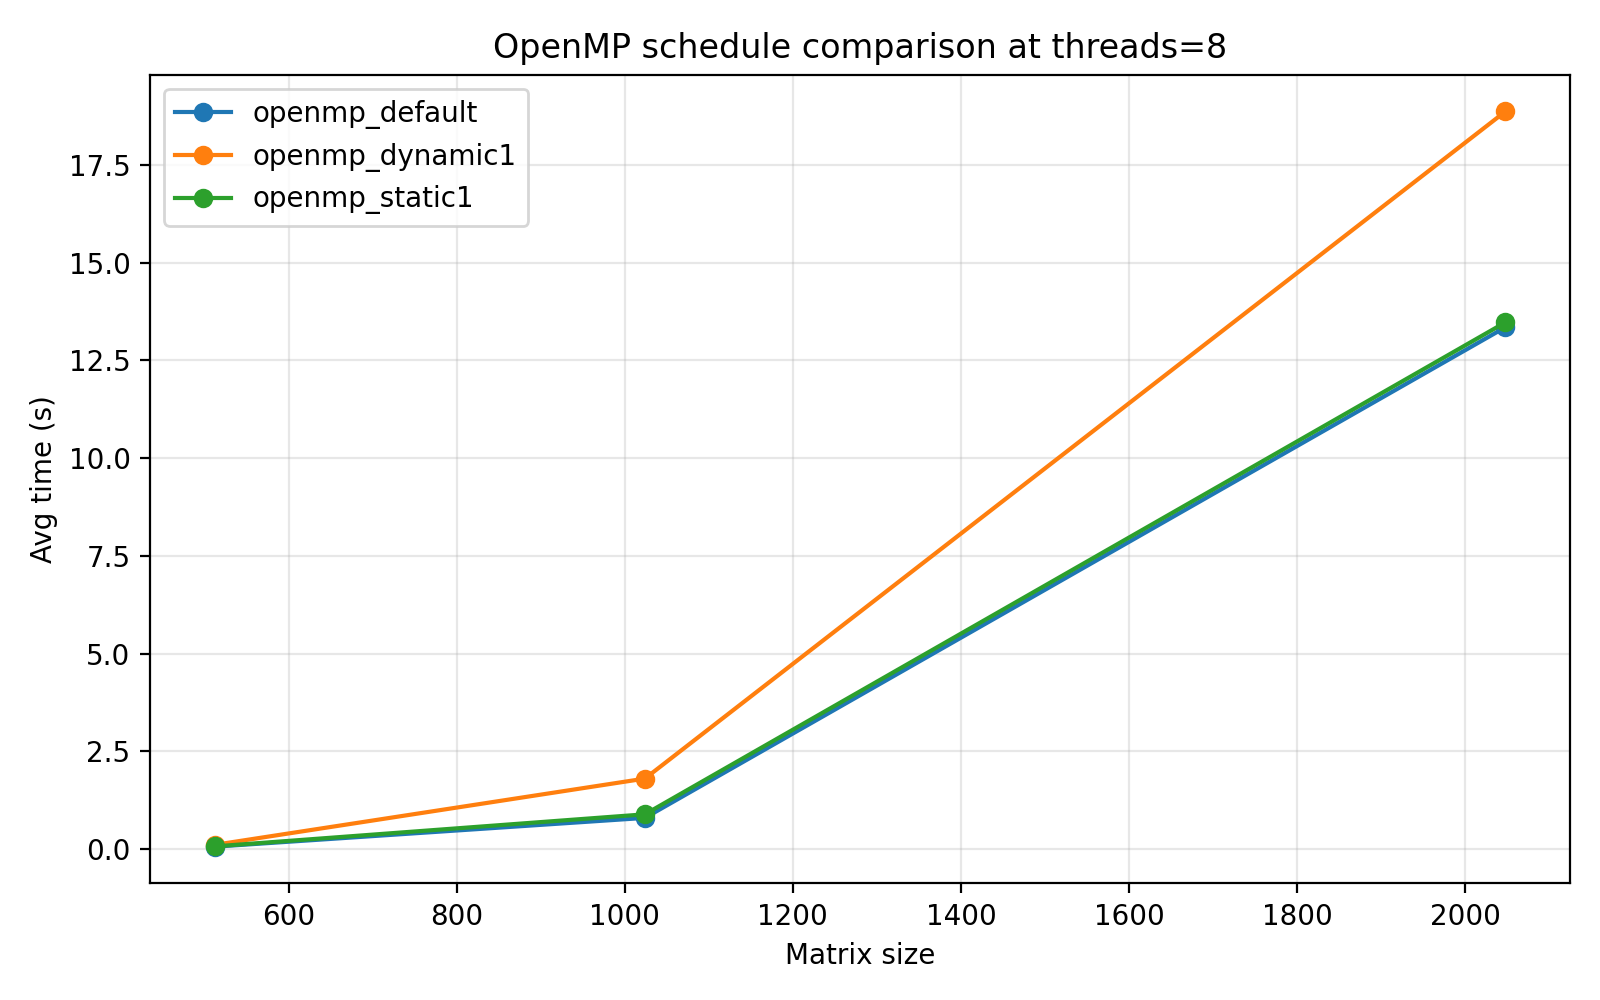
\includegraphics[width=0.85\textwidth]{openmp_schedule_comparison.png}
  \caption{OpenMP 三种调度策略对比}
\end{figure}

\begin{figure}[H]
  \centering
  \begin{subfigure}[t]{0.32\textwidth}
    \centering
    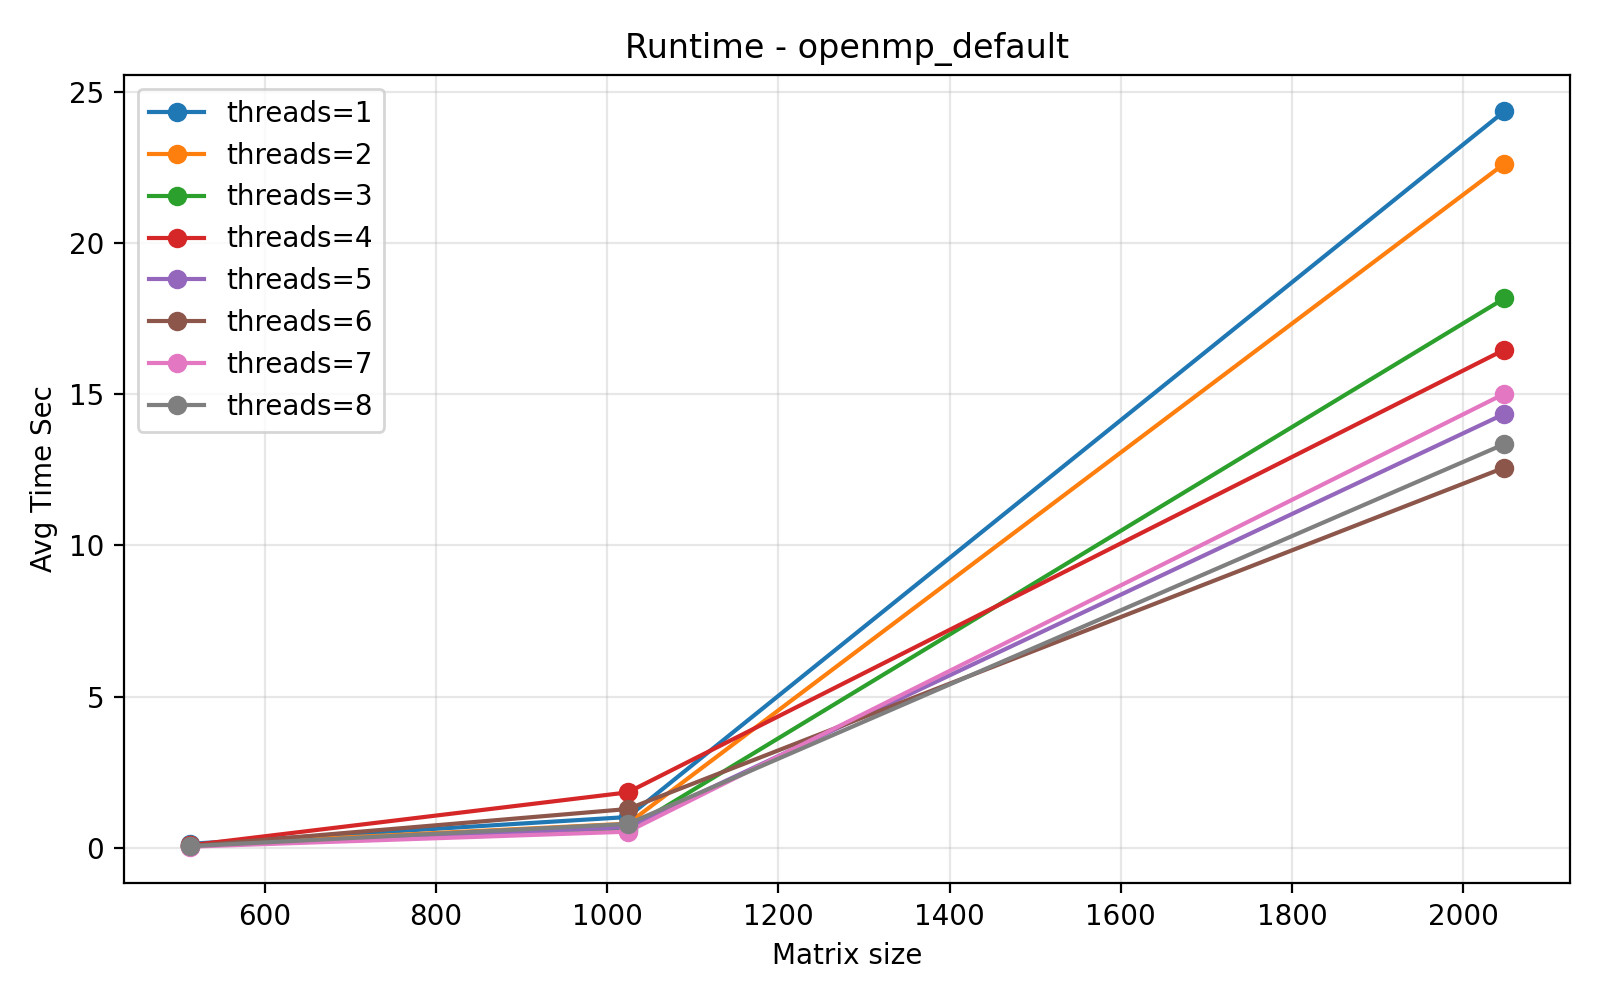
\includegraphics[width=\textwidth]{runtime_openmp_default.png}
    \caption{default}
  \end{subfigure}
  \hfill
  \begin{subfigure}[t]{0.32\textwidth}
    \centering
    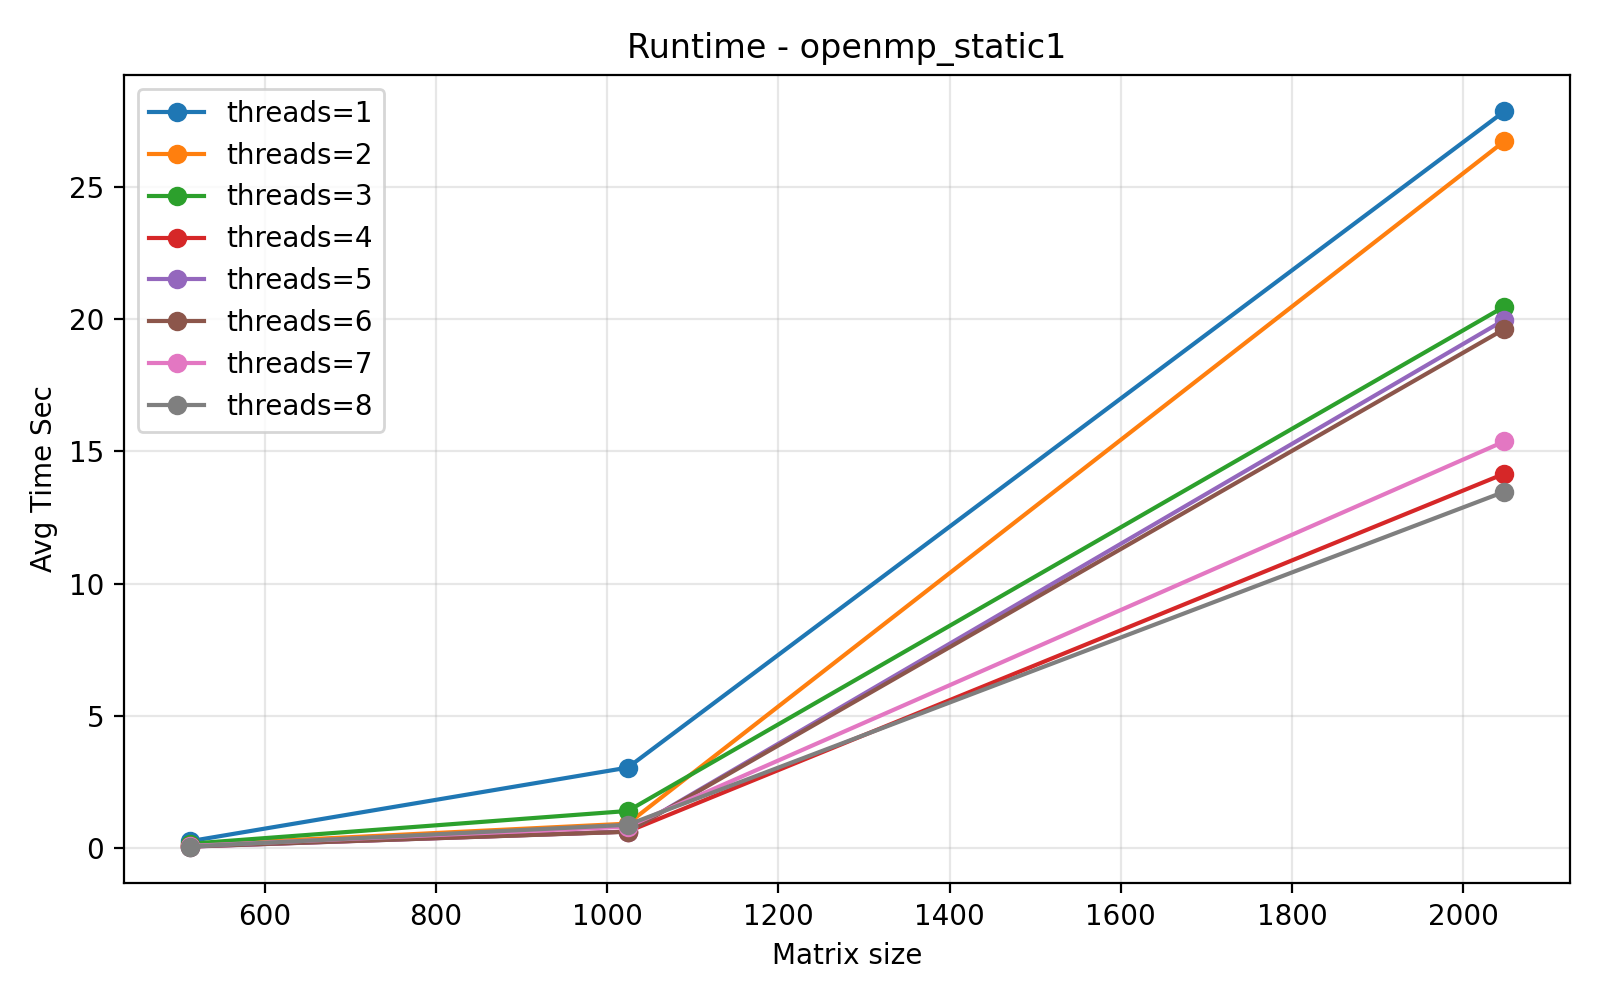
\includegraphics[width=\textwidth]{runtime_openmp_static1.png}
    \caption{static(1)}
  \end{subfigure}
  \hfill
  \begin{subfigure}[t]{0.32\textwidth}
    \centering
    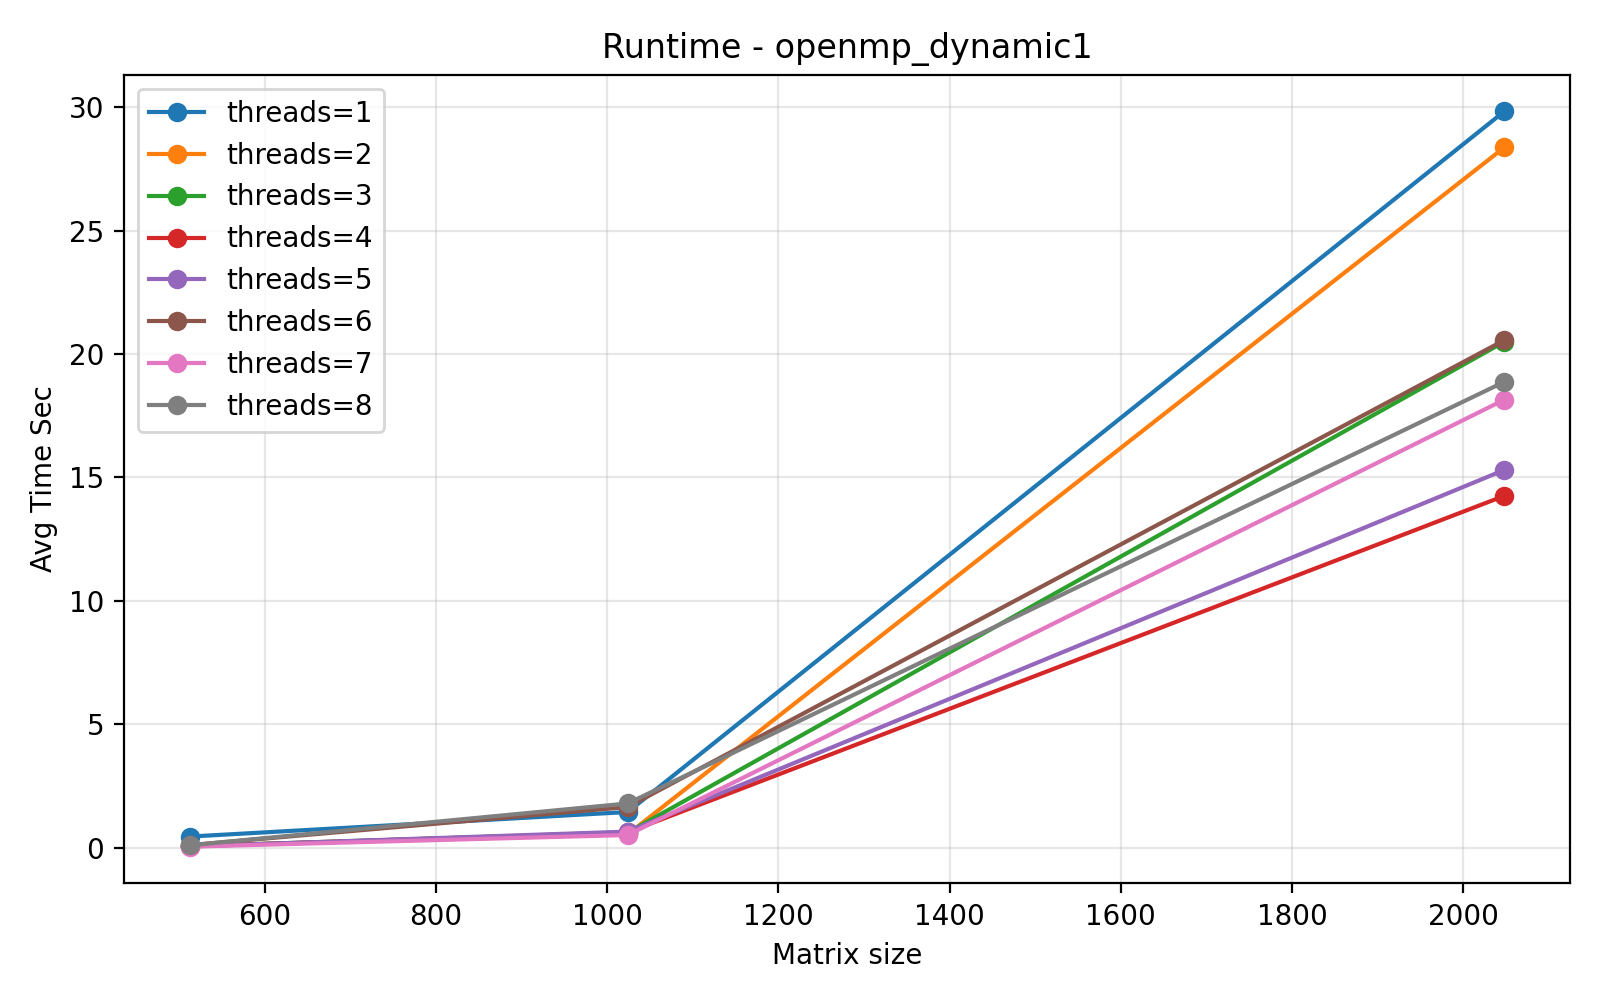
\includegraphics[width=\textwidth]{runtime_openmp_dynamic1.png}
    \caption{dynamic(1)}
  \end{subfigure}
  \caption{OpenMP 三种调度策略运行时间曲线}
\end{figure}

\begin{figure}[H]
  \centering
  \begin{subfigure}[t]{0.32\textwidth}
    \centering
    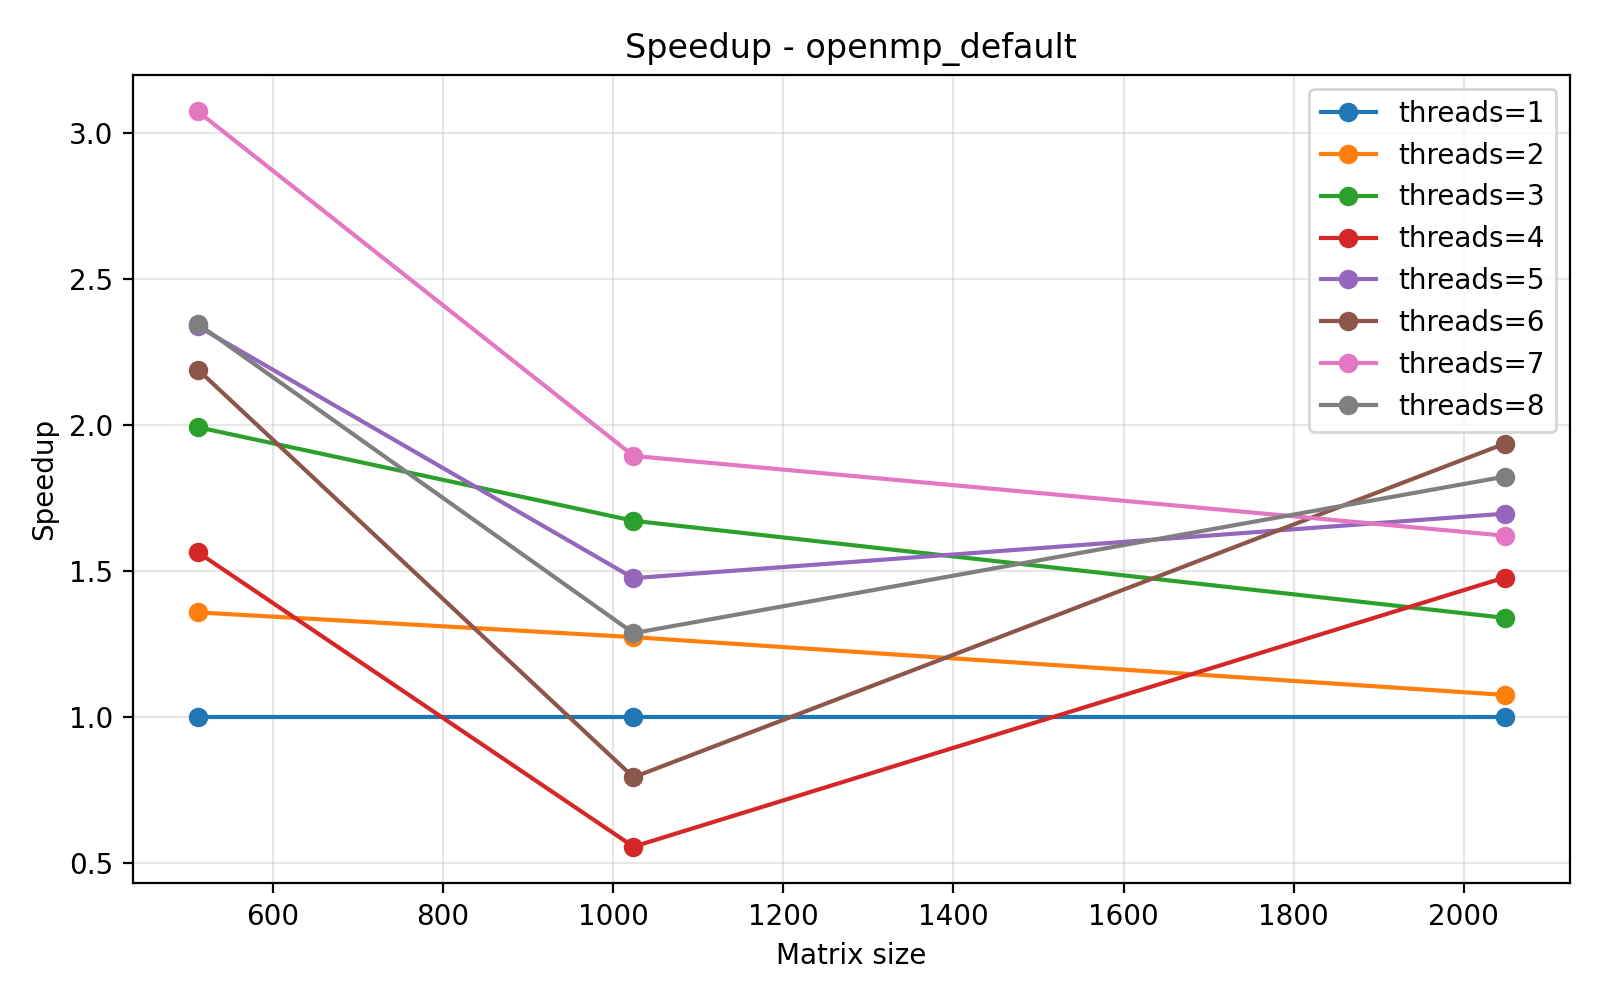
\includegraphics[width=\textwidth]{speedup_openmp_default.png}
    \caption{default}
  \end{subfigure}
  \hfill
  \begin{subfigure}[t]{0.32\textwidth}
    \centering
    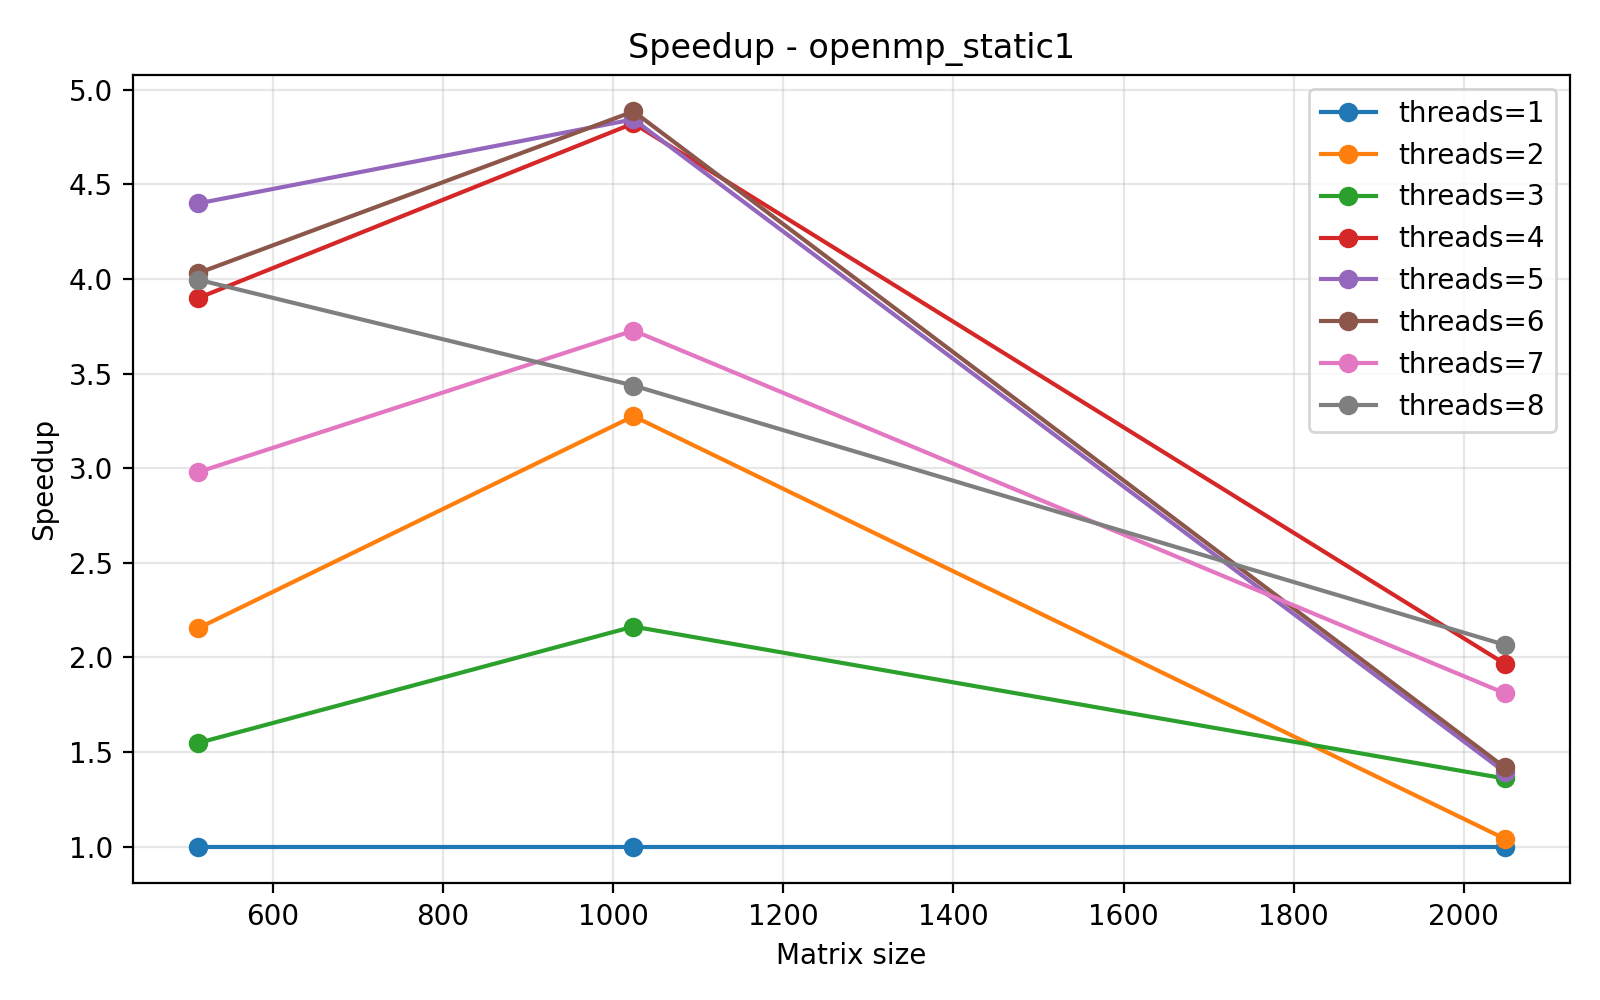
\includegraphics[width=\textwidth]{speedup_openmp_static1.png}
    \caption{static(1)}
  \end{subfigure}
  \hfill
  \begin{subfigure}[t]{0.32\textwidth}
    \centering
    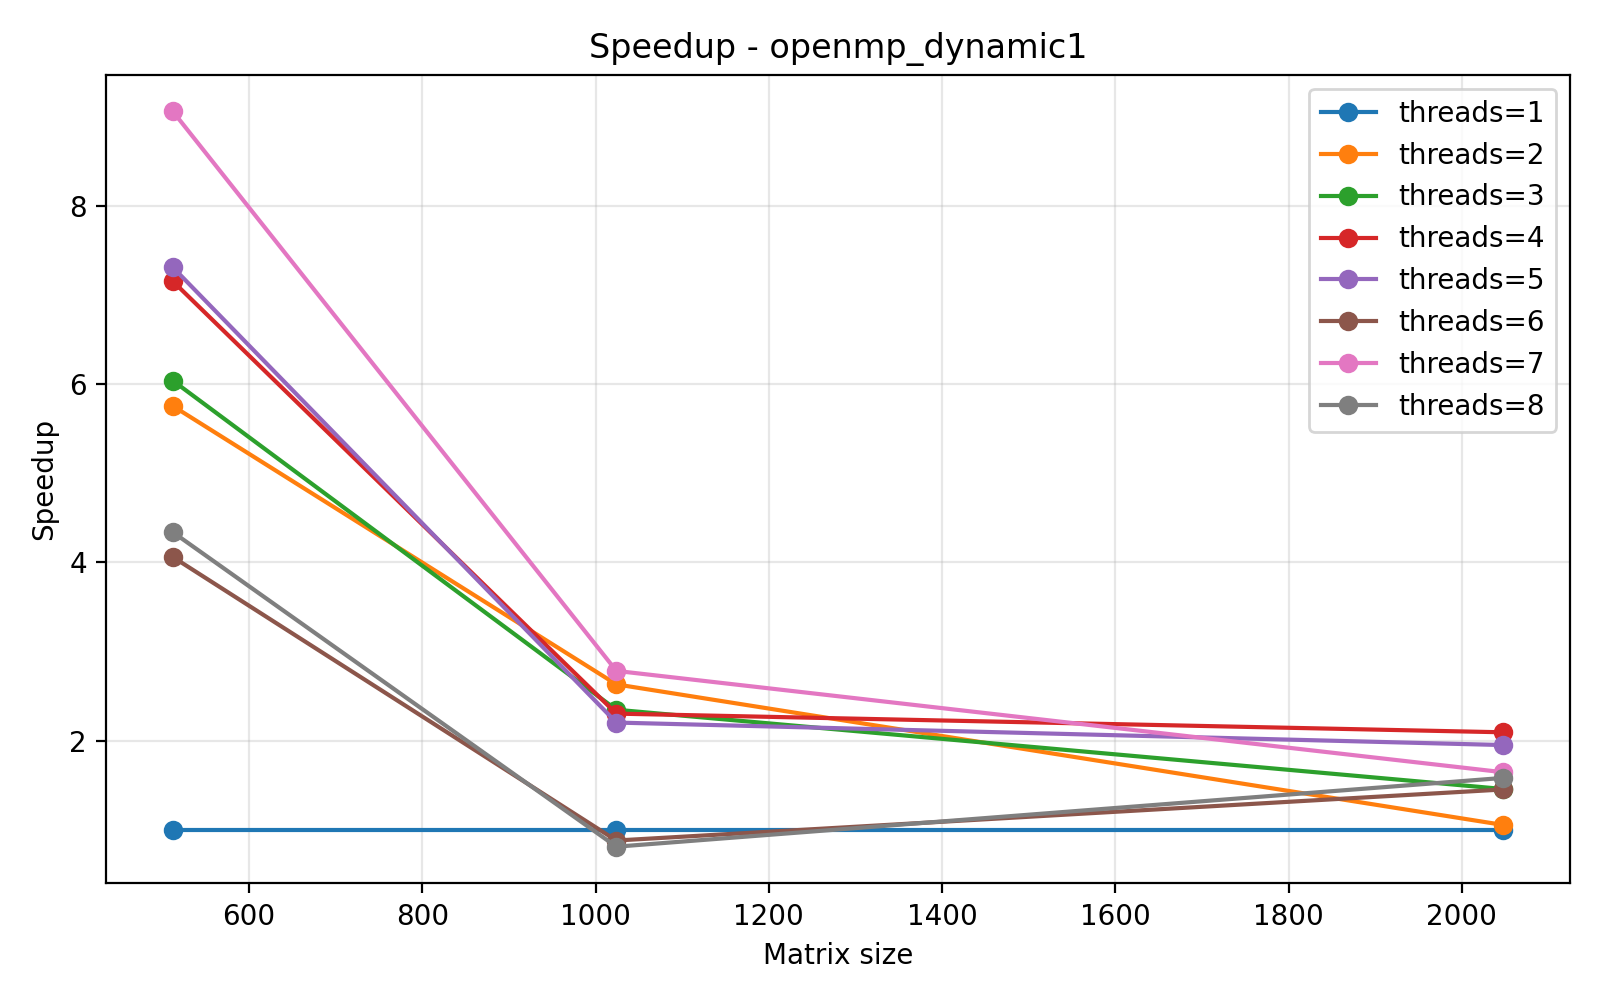
\includegraphics[width=\textwidth]{speedup_openmp_dynamic1.png}
    \caption{dynamic(1)}
  \end{subfigure}
  \caption{OpenMP 三种调度策略加速比曲线}
\end{figure}

\begin{figure}[H]
  \centering
  \begin{subfigure}[t]{0.32\textwidth}
    \centering
    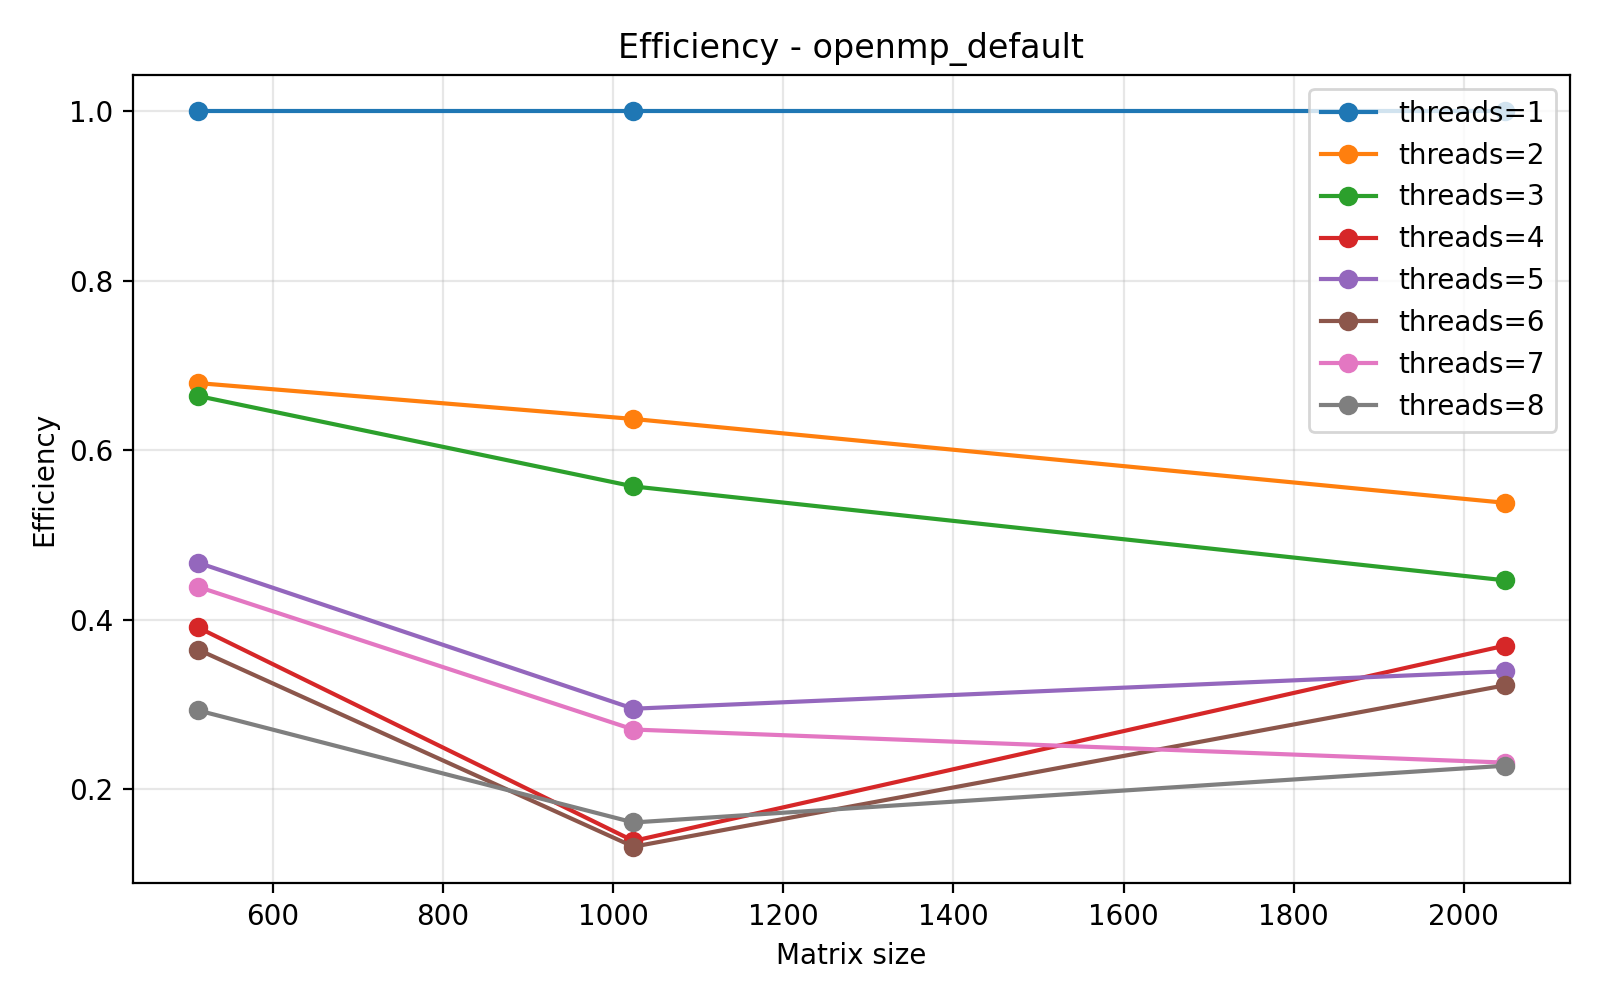
\includegraphics[width=\textwidth]{efficiency_openmp_default.png}
    \caption{default}
  \end{subfigure}
  \hfill
  \begin{subfigure}[t]{0.32\textwidth}
    \centering
    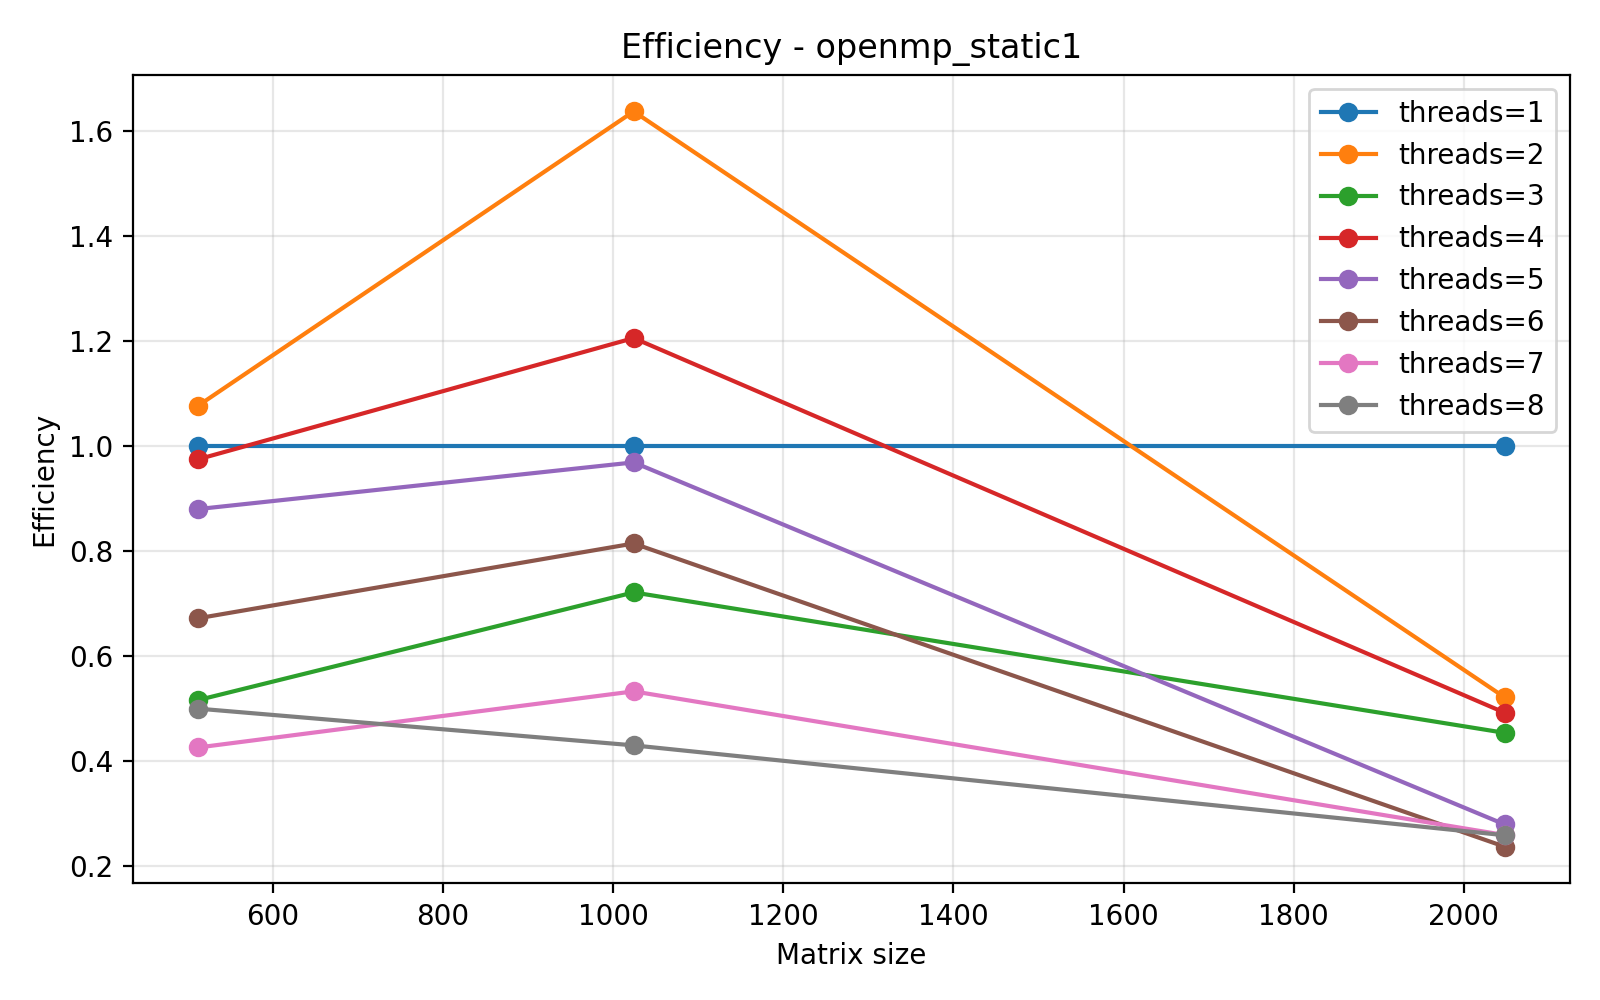
\includegraphics[width=\textwidth]{efficiency_openmp_static1.png}
    \caption{static(1)}
  \end{subfigure}
  \hfill
  \begin{subfigure}[t]{0.32\textwidth}
    \centering
    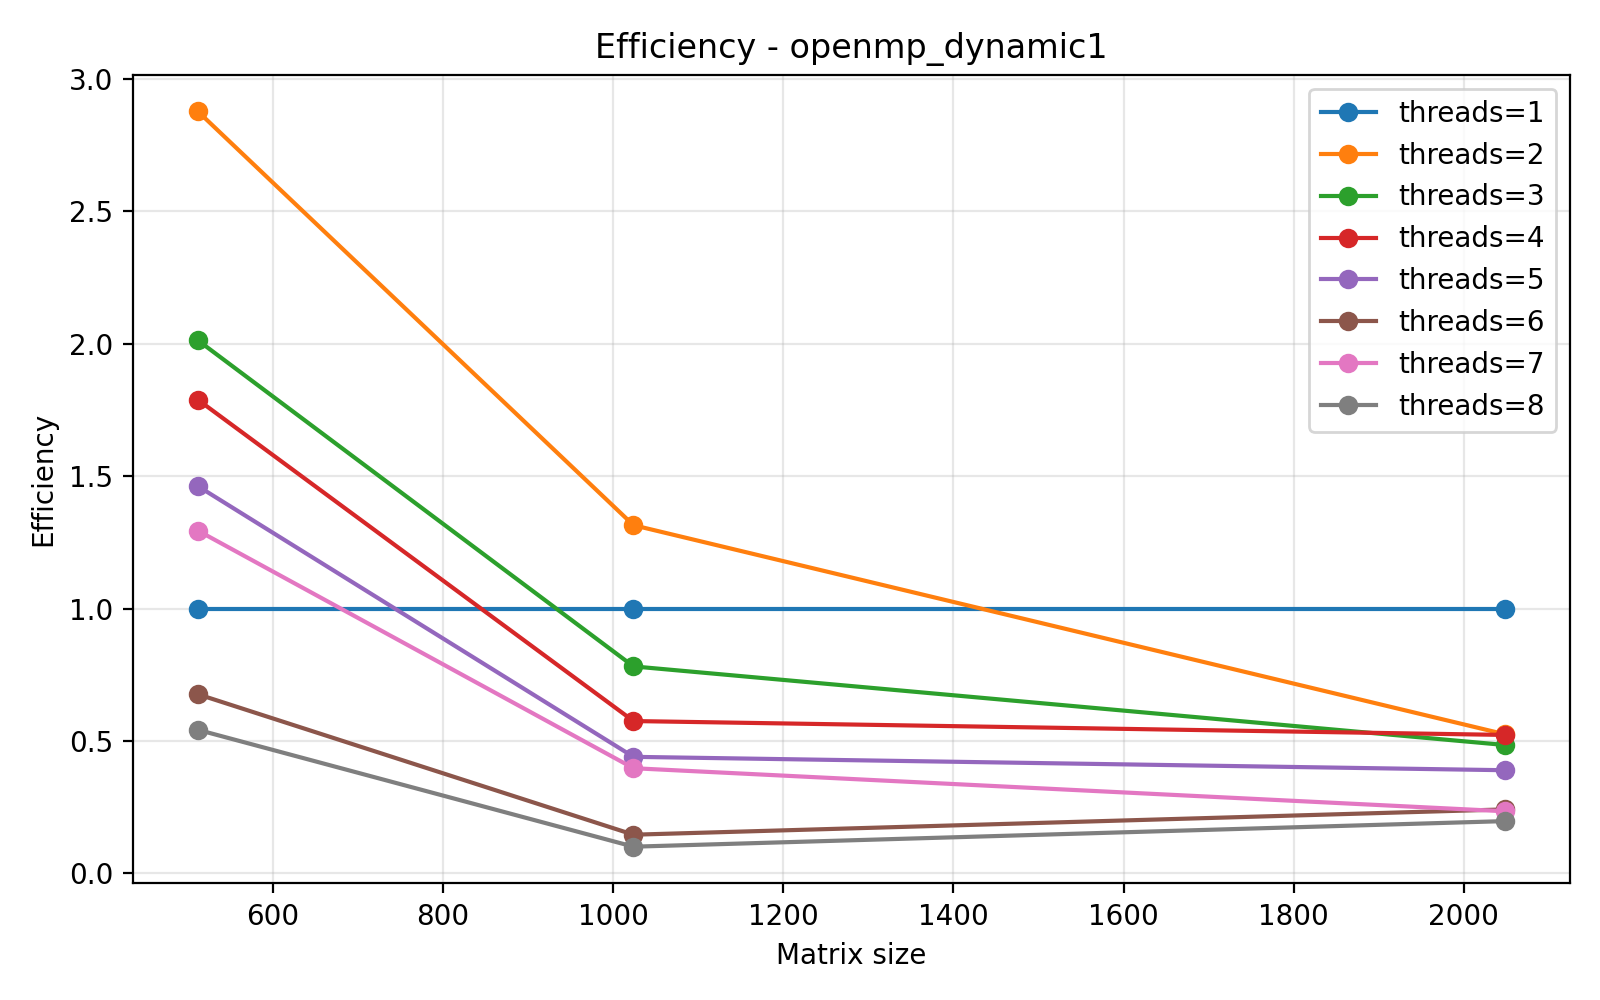
\includegraphics[width=\textwidth]{efficiency_openmp_dynamic1.png}
    \caption{dynamic(1)}
  \end{subfigure}
  \caption{OpenMP 三种调度策略并行效率曲线}
\end{figure}

\begin{figure}[H]
  \centering
  \begin{subfigure}[t]{0.32\textwidth}
    \centering
    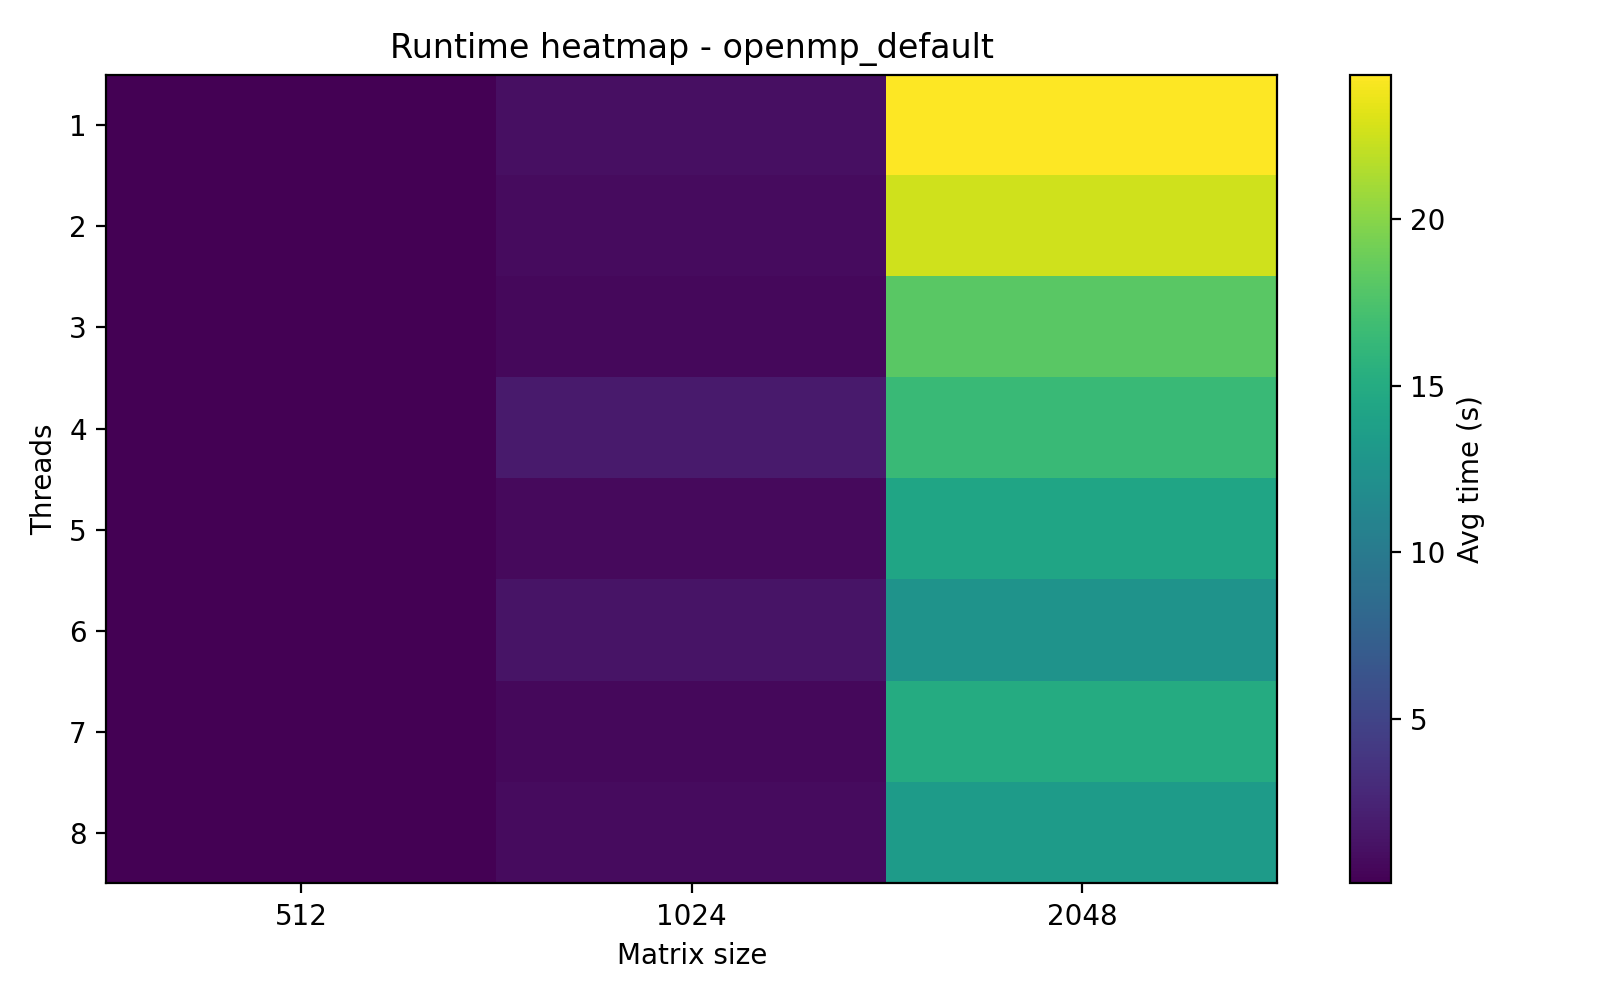
\includegraphics[width=\textwidth]{heatmap_openmp_default.png}
    \caption{default}
  \end{subfigure}
  \hfill
  \begin{subfigure}[t]{0.32\textwidth}
    \centering
    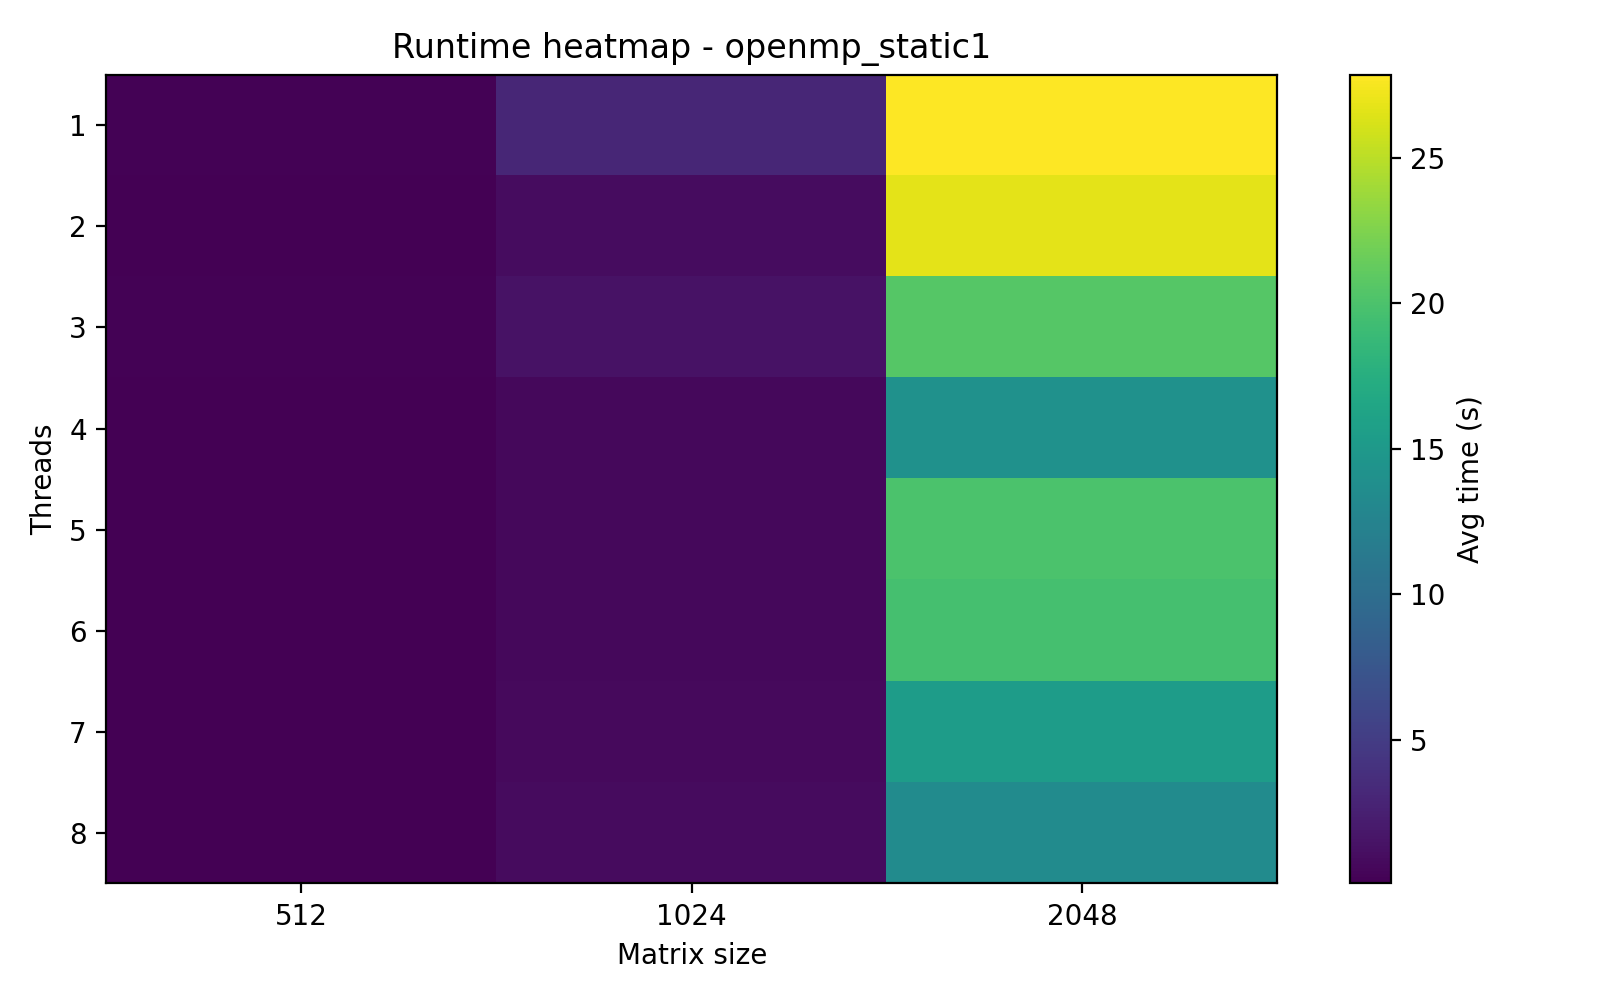
\includegraphics[width=\textwidth]{heatmap_openmp_static1.png}
    \caption{static(1)}
  \end{subfigure}
  \hfill
  \begin{subfigure}[t]{0.32\textwidth}
    \centering
    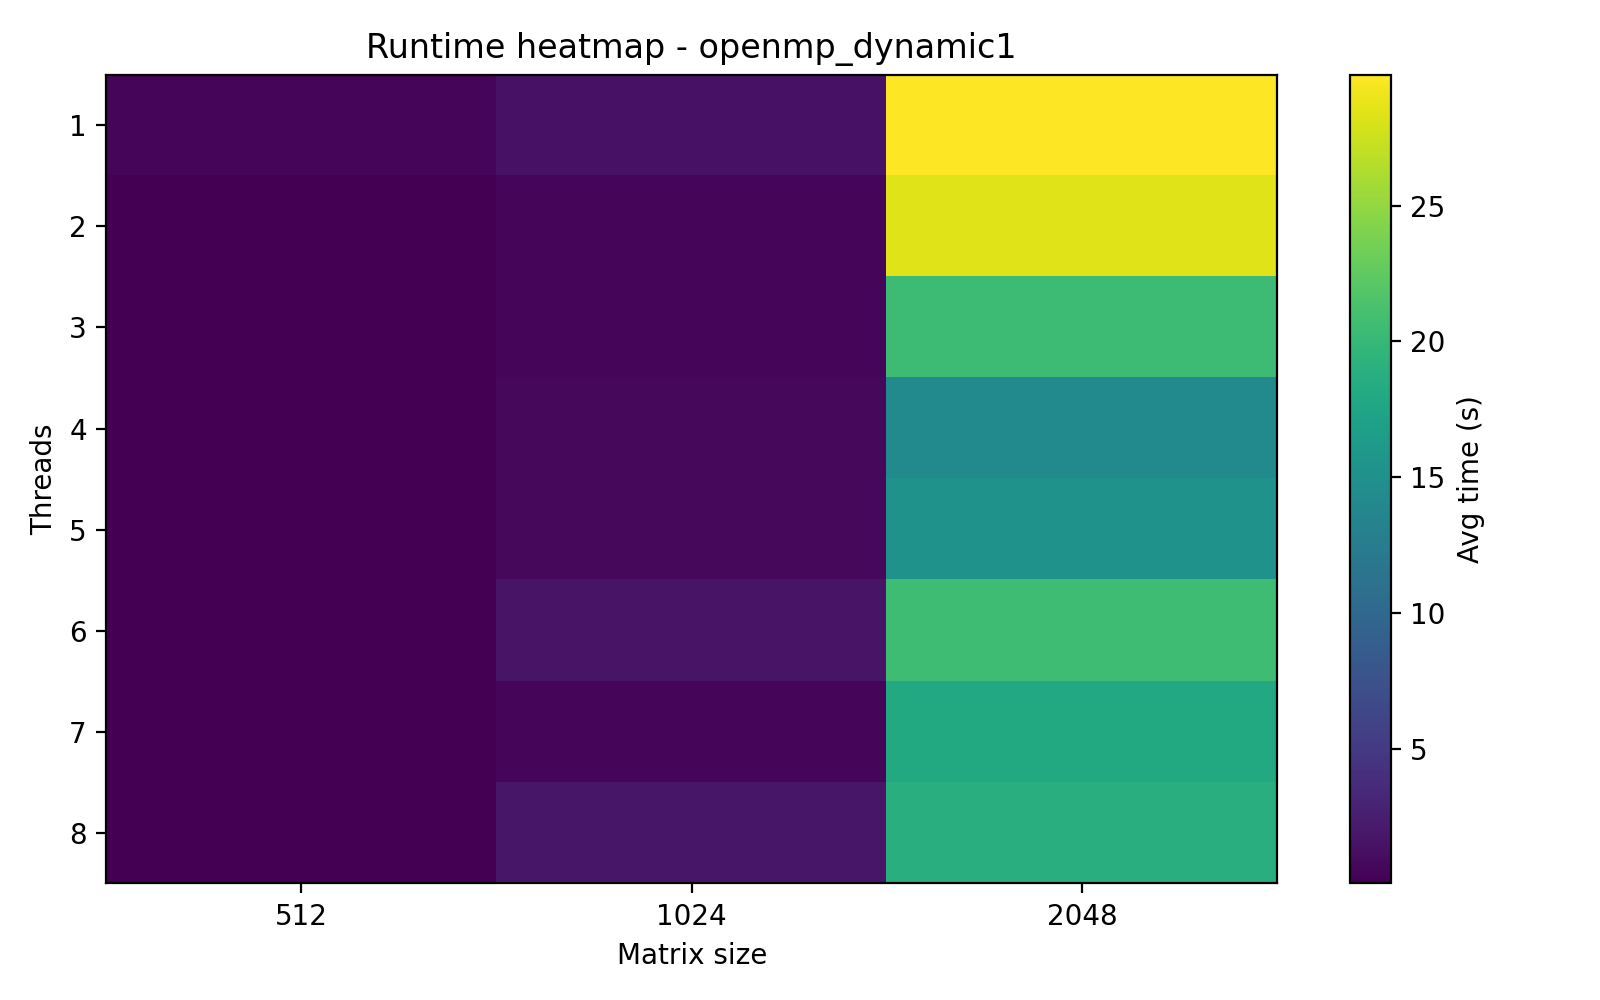
\includegraphics[width=\textwidth]{heatmap_openmp_dynamic1.png}
    \caption{dynamic(1)}
  \end{subfigure}
  \caption{OpenMP 三种调度策略热力图}
\end{figure}

\subsection{OpenMP 结果分析}

从 8 线程结果看，\texttt{openmp\_default} 在三个规模下都给出了最短运行时间：当矩阵规模为 512 时，\texttt{default}、\texttt{static(1)} 和 \texttt{dynamic(1)} 分别约为 0.0592s、0.0664s 和 0.1059s；当规模提升到 1024 时，三者分别约为 0.7956s、0.8873s 和 1.8009s；当规模为 2048 时，三者分别约为 13.3494s、13.4750s 和 18.8711s。可以看到，\texttt{static(1)} 在大规模下已经接近 \texttt{default}，而 \texttt{dynamic(1)} 在本实验这种规则、均匀的任务上始终更慢。

若只看 2048 规模下各版本的最佳线程配置，\texttt{openmp\_default} 在 6 线程时达到最优，为 12.5710s；\texttt{openmp\_static1} 在 8 线程时达到 13.4750s；\texttt{openmp\_dynamic1} 在 4 线程时达到 14.2550s。这个现象说明线程数不是单调收益源，线程继续增加后会受到调度、同步和内存带宽竞争影响，因此运行时间会出现波动。综合图和表来看，OpenMP 默认调度在本实验中最适合作为基线方案。

\subsection{\texttt{parallel\_for} 动态库验证}

\begin{figure}[H]
  \centering
  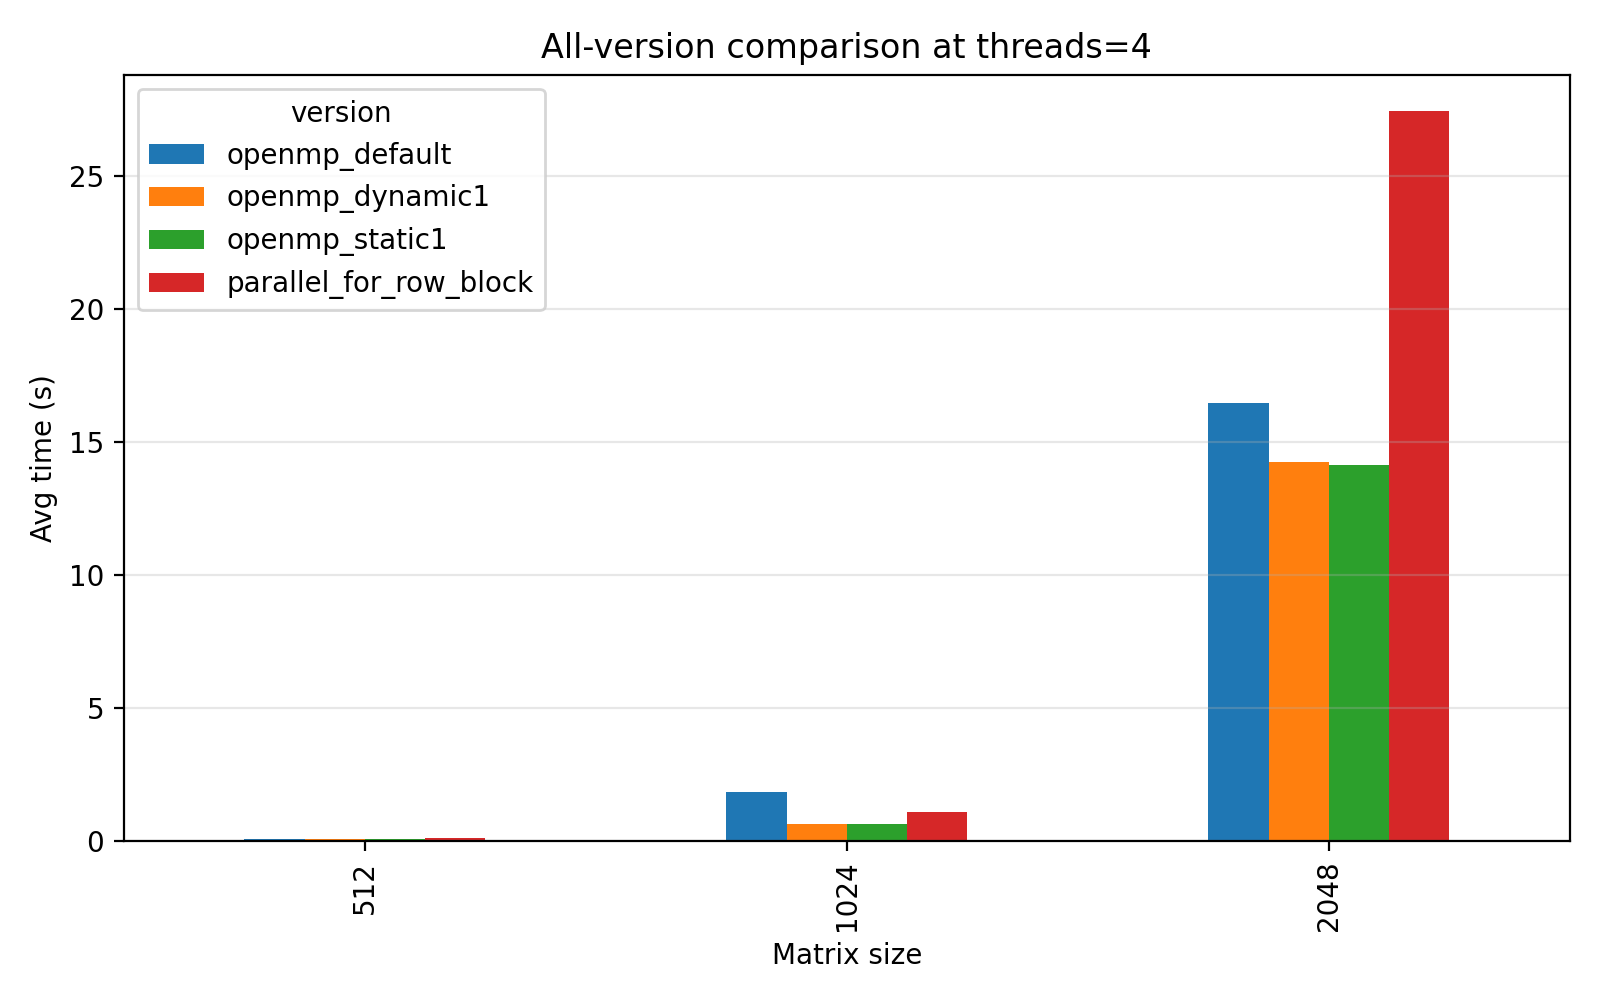
\includegraphics[width=0.85\textwidth]{version_comparison_all.png}
  \caption{全部版本在同一线程配置下的对比}
\end{figure}

\begin{figure}[H]
  \centering
  \begin{subfigure}[t]{0.48\textwidth}
    \centering
    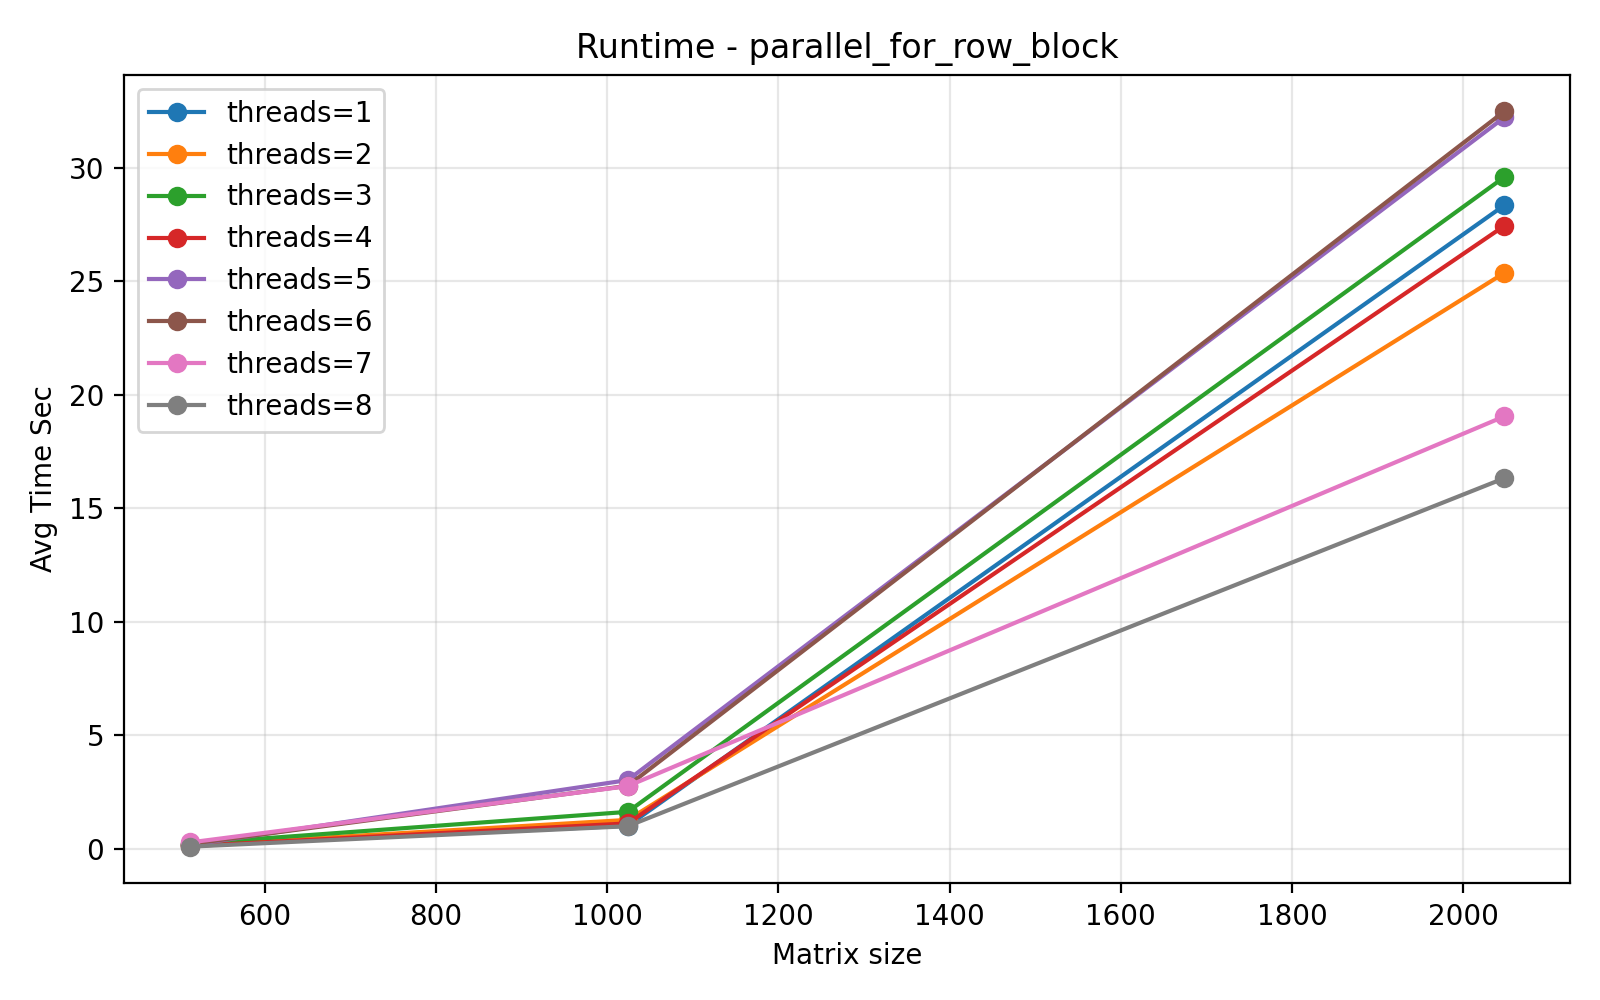
\includegraphics[width=\textwidth]{runtime_parallel_for_row_block.png}
    \caption{运行时间曲线}
  \end{subfigure}
  \hfill
  \begin{subfigure}[t]{0.48\textwidth}
    \centering
    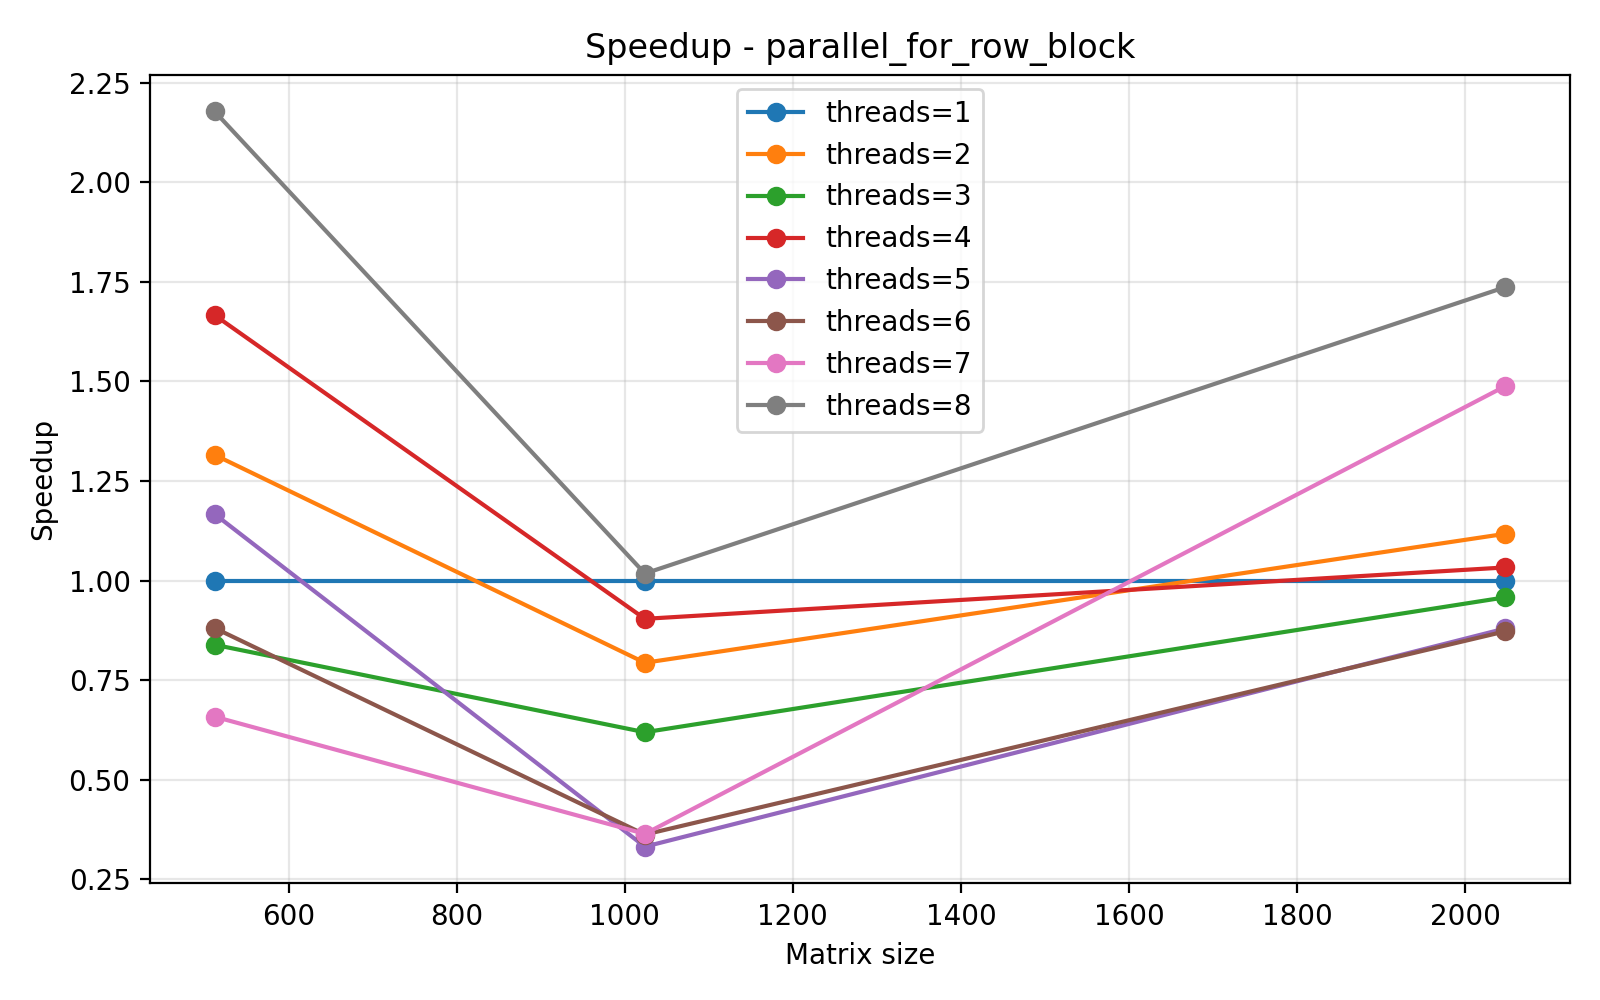
\includegraphics[width=\textwidth]{speedup_parallel_for_row_block.png}
    \caption{加速比曲线}
  \end{subfigure}
  \caption{\texttt{parallel\_for\_row\_block} 性能结果}
\end{figure}

\begin{figure}[H]
  \centering
  \begin{subfigure}[t]{0.48\textwidth}
    \centering
    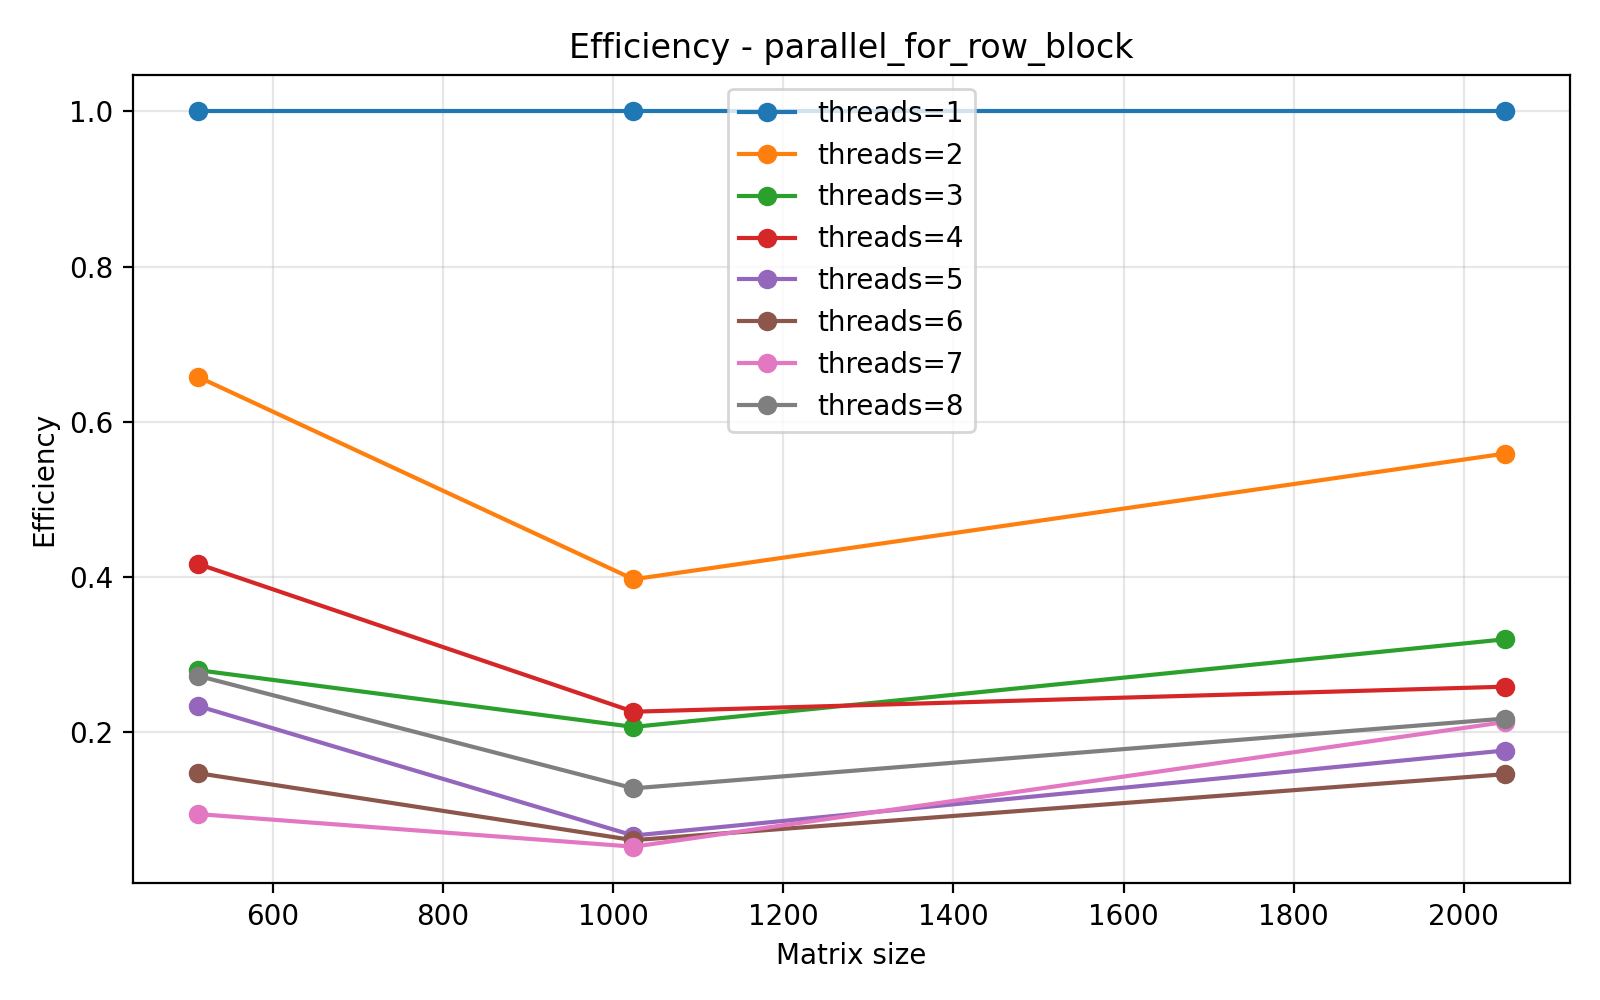
\includegraphics[width=\textwidth]{efficiency_parallel_for_row_block.png}
    \caption{并行效率曲线}
  \end{subfigure}
  \hfill
  \begin{subfigure}[t]{0.48\textwidth}
    \centering
    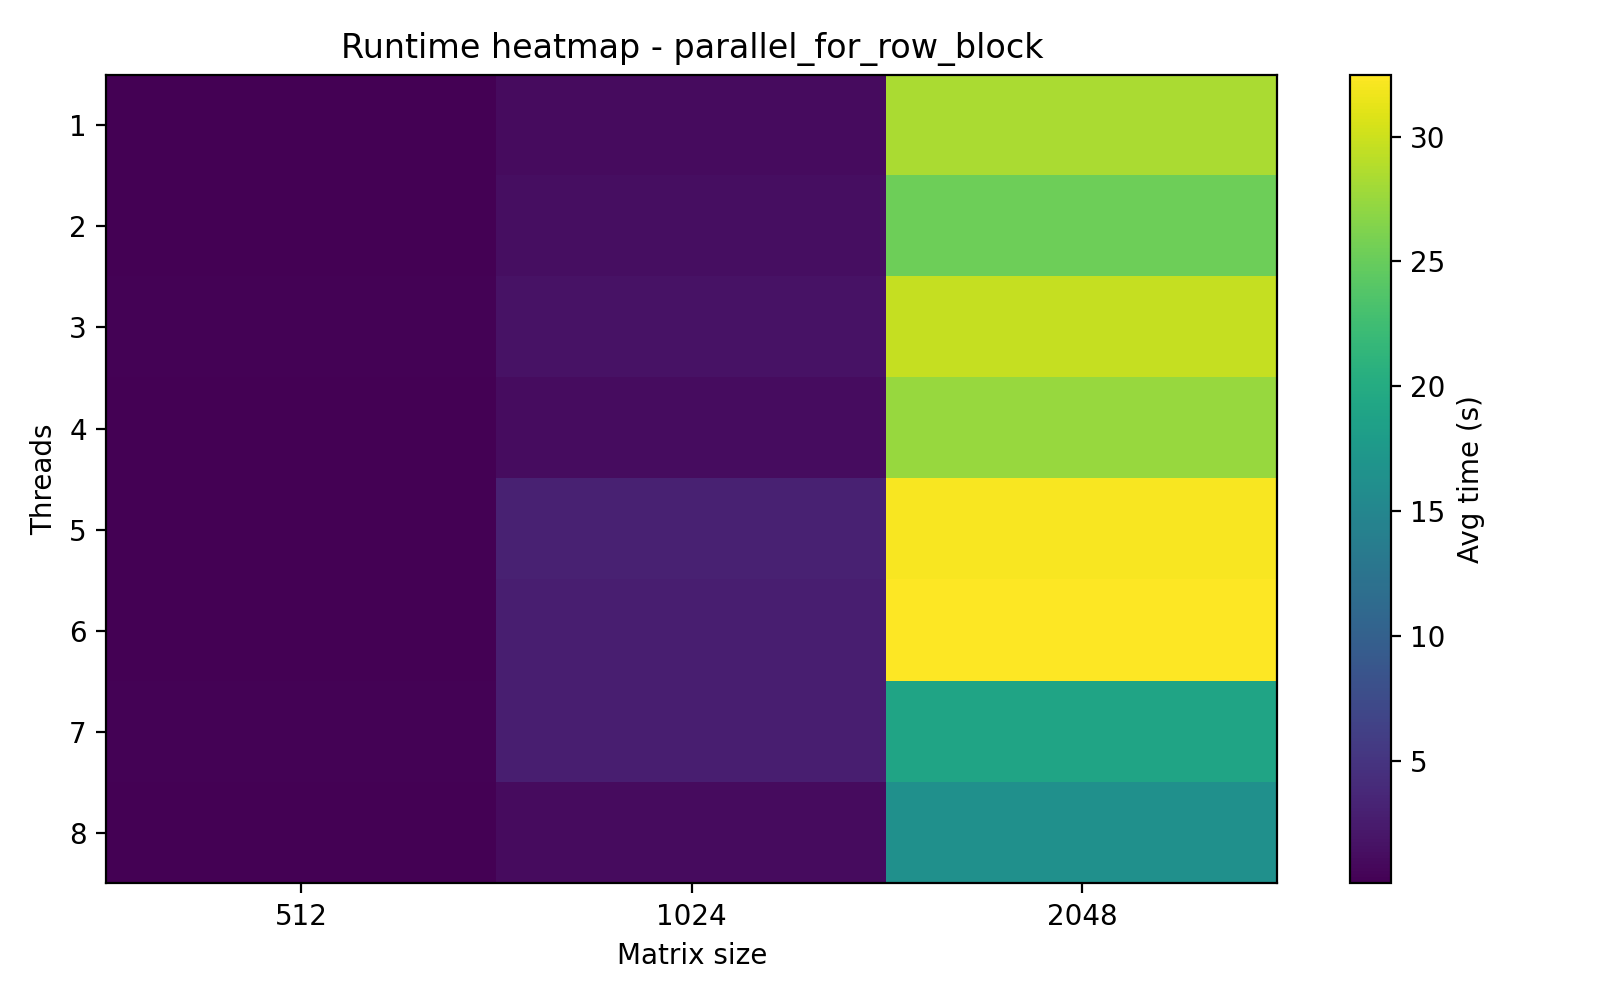
\includegraphics[width=\textwidth]{heatmap_parallel_for_row_block.png}
    \caption{热力图}
  \end{subfigure}
  \caption{\texttt{parallel\_for\_row\_block} 扩展特征}
\end{figure}

\subsection{\texttt{parallel\_for} 结果分析}

\texttt{parallel\_for} 动态库在 Docker Linux 环境中成功生成
\texttt{libparallel\_for.so}，并被 \texttt{parallel\_for\_matmul} 正常加载执行。
所有线程配置下的 \texttt{checksum} 与 OpenMP 三个版本保持一致，
说明基于 Pthreads 的并行 \texttt{for} 分解在正确性上是成立的。

从性能上看，该版本在 2048 规模下的单线程时间约为 28.3465s，
最佳结果出现在 8 线程，为 16.3184s，对应加速比约为 1.74。
相比之下，2 线程仅提升到约 25.3660s，3 到 6 线程阶段还出现了波动甚至退化，
直到 7 和 8 线程时才出现更明显的收益。
这说明当前实现虽然完成了并行划分与动态库调用要求，
但线程创建、销毁、同步以及连续块划分带来的负载不均和缓存竞争仍然比较明显，
因此扩展性弱于 OpenMP。

将 \texttt{parallel\_for} 与最佳 OpenMP 版本对比，在 2048 规模下，
\texttt{openmp\_default} 的最佳时间为 12.5710s，而该版本的最佳时间为 16.3184s，
后者明显更慢。这一结果符合预期：OpenMP 运行时本身已经对线程调度和并行循环
做了更成熟的优化，而本实验中的 \texttt{parallel\_for}
仅实现了最基础的连续块划分机制，因此它更适合作为
“并行 \texttt{for} 机制构造”的教学验证，而不是作为性能最优方案。

\section{性能结论汇总}

\begin{table}[H]
  \centering
  \small
  \caption{最终性能结论汇总}
  \renewcommand{\arraystretch}{1.18}
  \begin{tabularx}{0.96\textwidth}{>{\raggedright\arraybackslash}p{3.1cm} >{\centering\arraybackslash}p{1.8cm} >{\centering\arraybackslash}p{1.9cm} X}
    \toprule
    比较对象 & 代表配置 & 结果 & 结论 \\
    \midrule
    OpenMP 三种调度 & 8 线程，512 / 1024 / 2048 & default 均最快 & 默认调度在本实验中整体表现最好 \\
    default vs static(1) & 2048，8 线程 & 13.3494s vs 13.4750s & static(1) 已接近 default，但仍略慢 \\
    default vs dynamic(1) & 2048，8 线程 & 13.3494s vs 18.8711s & dynamic(1) 在规则任务上调度开销偏大 \\
    OpenMP 最佳配置 & 2048，全线程扫描 & default 在 6 线程达到 12.5710s & 线程数增加并非单调收益，存在最优点 \\
    \texttt{parallel\_for} 扩展性 & 2048，1 线程到 8 线程 & 28.3465s 降到 16.3184s & 能获得加速，但扩展效率明显弱于 OpenMP \\
    OpenMP vs \texttt{parallel\_for} & 2048，各自最佳结果 & 12.5710s vs 16.3184s & 手工构造并行 \texttt{for} 可行，但性能仍落后成熟运行时 \\
    \bottomrule
  \end{tabularx}
\end{table}

\section{结论}

本实验完成了两条主线任务：一是用 OpenMP 实现并比较三种矩阵乘法调度策略，二是构造基于 Pthreads 的 \texttt{parallel\_for} 动态库并用于矩阵乘法验证。实验结果表明，三种 OpenMP 版本和 \texttt{parallel\_for} 版本都能给出一致的数值结果，说明实现正确。

在性能方面，OpenMP 默认调度整体最好。\texttt{schedule(static,1)}
在大规模下与默认调度接近，但总体仍略慢；
\texttt{schedule(dynamic,1)} 由于调度开销较大，
在本实验这种规则任务上没有体现优势。

对于 \texttt{parallel\_for} 动态库，虽然它已经完成了 Linux \texttt{.so}
生成、外部程序调用和并行执行的要求，但其扩展效率弱于 OpenMP，
说明手工构造的基础版并行 \texttt{for} 机制在功能上可行，
在性能上仍有进一步优化空间。

\end{document}
